\documentclass[11pt,b5paper]{book}

\usepackage[utf8]{inputenc}

\usepackage{graphicx} % [draft]{graphicx} to remove all images
\graphicspath{ {images/} }
\usepackage{wrapfig}

\usepackage{breakcites}

\usepackage[strict]{changepage} % for CV. As the "section" of bch font is slightly off the balance compared with "main text" of crimson font. the balance is then fixed by placing the bch font in the main text, and the "section" of bch font is adjusted accordingly.

%=======================================================================
%%% thesis geometry

\usepackage[text={115mm,197.2mm},hmarginratio=1:1,vmarginratio=1:1,marginparwidth=12mm]{geometry} 

%=======================================================================

\usepackage{lipsum} %generating lorem ipsum

\usepackage{amsmath,amssymb,amsfonts}

\usepackage{setspace}
\usepackage{booktabs}

\usepackage{emptypage} %remove header, footer along with the page number in an empty page
\newcommand\mybar{\kern1pt\rule[-\dp\strutbox]{1pt}{\baselineskip}\kern1pt} %vertical bar
\usepackage{pdfpages} %[draft]{pdfpages} to remove all pdf

\usepackage{float} %force image position

\usepackage{url}
\urlstyle{same}

\usepackage[super]{nth}

\usepackage{textgreek}

\usepackage[hang,flushmargin]{footmisc}
\renewcommand*{\footnotelayout}{\scriptsize}

\usepackage{multirow}

\usepackage[many,listings]{tcolorbox} % color box surrounding anything

%=======================================================================
%%% Minimize overfull hbox output problem

\usepackage{microtype}

%=======================================================================
%%% Abbreviations and add this section to table of contents

\usepackage{multicol} % multicolumns

\usepackage[intoc]{nomencl}
\usepackage{ifthen}
\setlength{\nomitemsep}{-2pt} % this modifies item vertical separation
\setlength{\nomlabelwidth}{1.6cm} % this modifies label horizontal separation; {2.5cm} for single column; {1.8cm} for two column, long acronyms

%%% Grouped multi-column nomenclature %%%

\makenomenclature

\setlength{\columnsep}{1.67pc} % column separation

\makeatletter
\newif\if@nomlist

\newcommand*\nomlist{%
  \@nomlisttrue
  \list{}{%
    \labelwidth\nom@tempdim
    \leftmargin\labelwidth
    \advance\leftmargin\labelsep
    \itemsep\nomitemsep
    \let\makelabel\nomlabel}}

\renewcommand*\thenomenclature{%
  \@ifundefined{chapter}%
    {\section*{\nomname}\if@intoc\addcontentsline{toc}{section}{\nomname}\fi}%
    {\chapter*{\nomname}\if@intoc\addcontentsline{toc}{chapter}{\nomname}\fi}%
  \nompreamble
  \@nomlistfalse
}

\renewcommand\nomgroup[1]{%
  \if@nomlist\endlist\end{multicols}\fi
  \ifx#1A\relax % "1A" can't be replaced with "1a". "a" is fine though in the nomenclature.tex
    \def\nomgroupname{\textbf{Acronyms}}%
  \else
    \ifx#1B\relax % "1B" can't be replaced with "1b". "b" is fine though in the nomenclature.tex
      \def\nomgroupname{\textbf{Roman symbols}}%
    \else
      \def\nomgroupname{\textbf{Greek symbols}}%
    \fi
  \fi
  \begin{multicols}{2}[\raggedcolumns\noindent\textbf{\hspace*{-1pt}\fontfamily{bch}\selectfont\scshape\small{\nomgroupname}}]
  \nomlist
}

\renewcommand*\nompreamble{}
\renewcommand*\nompostamble{\end{multicols}}
\makeatother

%=======================================================================
%%% Modifying the listing items

\usepackage{enumitem}  
\usepackage{pgfornament}
\usepackage{adforn}

%=======================================================================
%%% Unique colors used in this PhD thesis
\usepackage{xcolor}
\definecolor{sophia}{RGB}{125,0,45}
\definecolor{ntnu}{RGB}{0,80,158}
\definecolor{heidelberg}{RGB}{0,65,120} % 

\usepackage{colortbl} % coloring the table
\definecolor{Gray}{gray}{0.9}
\definecolor{White}{RGB}{255,255,255}

% for abstract in chapters 5-9
\definecolor{abstractback}{RGB}{255,248,220}

\definecolor{Test}{RGB}{231,231,231} % must be CAPITALIZED!!!
\definecolor{Test3}{RGB}{128,128,128}
\definecolor{Black}{RGB}{0.0, 0.0, 0.0}
% for figure & table captions, marginnote, etc

\newcommand{\sophia}[1]{\textcolor{sophia}{#1}}
% too late, only used in Acknowledgement

%=======================================================================
%%% hyperref

\usepackage[backref=page]{hyperref}

\hypersetup{
    hidelinks,
    colorlinks=true,
    linkcolor=ntnu,
    citecolor=ntnu,
    urlcolor=ntnu,
    breaklinks,
    linktocpage % for TITLETOC: need to use this to make page number, not text be linked (automatically colored to "ntnu"). if this option is not used, then any text in toc or lof can't be customized in TITLETOC.
}

% === back references == 

\newcommand{\citedbox}[1]{%
  \begingroup\setlength{\fboxsep}{1pt}% 1pt is the default value; height
  \colorbox{White}{\hspace*{-1pt}\vphantom{Ay}#1\hspace*{-1pt}}% each 2pt is the default value; width
  \endgroup % originally the colorbox is set to "Test". it is good, but draws too much attention.
}

\usepackage{etoolbox}

\def\backref#1{{\citedbox{\textcolor{Test3}{Cited on page/s} #1\textcolor{Test3}{.}}}} % use this when \citedbox command is used. 

% === \ref = \autoref == %

%% to make the word "Figure" clickable in addition to its number label
\makeatletter
\renewcommand{\p@figure}{\figurename\ }
\makeatother

%% to make the word "Table" clickable in addition to its number label
\makeatletter
\renewcommand{\p@table}{\tablename\ }
\makeatother

% === explicitly mention the Section name === %

\newcommand*{\fullref}[1]{\hyperref[{#1}]{\autoref*{#1} \nameref*{#1}}}

\renewcommand{\sectionautorefname}{Section}

% ======================== %

%%% Capitalize [C]hapter, [S]ection and [S]ubsection in \autoref (default is not capitalized)

\newcommand{\Autoref}[1]{%
  \begingroup%
  \def\chapterautorefname{Chapter}%
  \def\sectionautorefname{Section}%
  \def\subsectionautorefname{Subsection}%
  \autoref{#1}%
  \endgroup%
}

%=======================================================================

\usepackage{bookmark} % Adding package bookmark improves bookmarks handling, and enable \pdfbookmark for TOC in the main.tex.

% add #(number) in front of the chapter title when it is exported to pdf

\bookmarksetup{numbered}

\makeatletter
\bookmarksetup{%
  addtohook={%
    \ifnum\toclevel@chapter=\bookmarkget{level}\relax
      \renewcommand*{\numberline}[1]{#1. }%
    \fi
  },
}
\makeatother

%=======================================================================
%%% Fonts used in this PhD thesis

\usepackage[T1]{fontenc}

\usepackage{csquotes}
\usepackage[english]{babel}

%% serif, as a main font %%
\usepackage{crimson}

%% sans serif, as decoration %%
\usepackage{roboto} %figure caption fonts

% math font
\usepackage[libertine]{newtxmath} 

% calligraphical font
\usepackage{calligra}

% hiragana/kanji
\usepackage{CJKutf8}

%=======================================================================
%%% Placing any extra information on the margin of the page

\usepackage{marginnote}

\renewcommand{\marginfont}{\fontsize{6.97}{6}\selectfont\roboto}

\newcounter{mynote}% a new counter for use in margin notes
 
\newcommand{\mynote}[2][0]{% a simple margin note
    \refstepcounter{mynote}% step counter
    \mbox{\textcolor{Test3}{\textsuperscript{\themynote}}}% the number (superscript) in text
    \marginnote{\mbox{\textcolor{Test3}{\textsuperscript{\themynote}}}\hspace{0pt}#2}[#1\baselineskip]% the note
    % \marginnote{\mbox{\textsuperscript{\themynote}}\color{sophia}\hspace{0pt}#2}[#1\baselineskip]% the note
}

\newcommand{\mynoteref}[2][0]{% a simple margin note
    \marginnote{\hspace{0pt}#2}[#1\baselineskip]% the note
}


% coloring the page number (referencing) in the copyright
\newcommand{\colpageref}[1]{{\hypersetup{linkcolor=sophia}{\pageref{#1}}}} % or \autopageref

% coloring the word "page" (referencing) in the copyright
\newcommand{\pcol}[1]{{\textcolor{Test3}{#1}}}

% to have a shortcut for coloring the caption, e.g., a, b, c, etc
\newcommand{\capcol}[1]{{\textcolor{ntnu}{#1}}}

%=======================================================================
%%% Bibliography at the end of each chapter, based on NATBIB

\usepackage[super,comma,sort&compress]{natbib} 

\usepackage{bibentry}

\usepackage[sectionbib]{chapterbib} % put ref at the end of each chapter. however, the spacing in the TOC will be messed up. it can be fixed using "numbib" option as shown below
\usepackage[nottoc,numbib]{tocbibind} % numbib (for numbering reference section) is used to enable cross-ref with TOC

\usepackage{hypernat} % to fix the missing page citation "\usepackage[backref=page]{hyperref}" that is nested in between, e.g., 19 is not missing if the refs is from 18-20, i.e., "sort&compress" in natbib is activated

\addto{\captionsenglish}{% if BABEL is used
  \renewcommand{\bibname}{References}
}

\renewcommand*{\bibfont}{\footnotesize}

\setlength{\bibsep}{0.7pt}

%=======================================================================
%=======================================================================
%=======================================================================
%%% Header (and/or footer)
%=======================================================================
%=======================================================================
%=======================================================================

\usepackage{fancyhdr}
\pagestyle{fancy} % this must be placed as a general. DON'T REMOVE IT!

%% with number in front of the title
\renewcommand{\chaptermark}[1]{ \markboth{Chap. \thechapter\ \ \enspace #1}{} } %\chaptername or "Chap."
\renewcommand{\sectionmark}[1]{ \markright{\thesection\ \ \quad #1} }

%==========================================================================%
%=================== header style for regular section =====================%
%==========================================================================%

\newcommand\headerregularsection{

    \pagestyle{fancy} % optional, but I place this here anyway
    \fancyhf{}

    \fancyhead[LE]{\leavevmode\llap{\textbf{\fontfamily{ppl}\selectfont\footnotesize\thepage} \ \hspace{1mm} \textcolor{sophia}{$\blacktriangleright$} \hspace{2mm}}{\scriptsize\bfseries\fontfamily{bch}\selectfont\scshape\leftmark}} % default font is Crimson for page number and Charter "bch" for the rest

    \fancyhead[RO]{{\scriptsize\bfseries\fontfamily{bch}\selectfont\scshape\rightmark}\rlap{\hspace{2.0mm} \textcolor{sophia}{$\blacktriangleleft$} \hspace{1mm} \ \textbf{\fontfamily{ppl}\selectfont\footnotesize\thepage}}} % default font is Crimson for page number and Charter "bch" for the rest

}

\setlength{\headheight}{13.6pt} % remove headheight error message: https://tex.stackexchange.com/questions/271159/turn-off-fancyhdr-auto-spacing, https://latex.org/forum/viewtopic.php?t=30693 

\renewcommand{\headrulewidth}{0pt}

%==========================================================================%
%=================== footer style for new chapter page ====================%
%==========================================================================%

\fancypagestyle{plain}{% % this command to set aside every new chapter to be different
    \fancyhf{}%
    \rfoot{\mypage} % draw box surrounding page
    \newcommand\mypage{%%
        \raisebox{6pt}[0pt][0pt]{%% {Xpt}[Xpt] determines the +y,-y both for the box AND the page number
        \color{ntnu}
        \rule[-1.5ex]{2.5cm}{0.5pt}%% [Xex]{Xcm}{Xex} are y position, the length of the box, work only with positive number and height of the box
        \hspace*{-2.0cm}%% box coordinate, right side
        \makebox[0pt]{\textcolor{ntnu}{\fontfamily{ppl}\selectfont\bfseries\footnotesize\thepage}}%% % page number properties ;  % default font is Crimson for page number and Charter "bch" for the rest
        \hspace*{0.5cm}}%% box coordinate, left side [BETTER not to change this]
    }        
    \fancyfootoffset{1.35\marginparwidth} % give offset to page number
}

%==========================================================================%
%========= header style for special section (a.k.a. REFERENCES) ===========%
%==========================================================================%

\newcommand\headerspecialsection{%
    \pagestyle{fancy} % fancypagestyle{CUSTOM_NAME}{} only work in the first page
    \fancyhf{}
    \fancyhead[LE]{\leavevmode\llap{\textbf{\fontfamily{ppl}\selectfont\footnotesize\thepage} \ \hspace{1mm} \textcolor{sophia}{$\blacktriangleright$} \hspace{2mm}}{\scriptsize\bfseries\fontfamily{bch}\selectfont\scshape\nouppercase\leftmark}} % default font is Crimson for page number and Charter "bch" for the rest

    \fancyhead[RO]{{\scriptsize\bfseries\fontfamily{bch}\selectfont\scshape\nouppercase\rightmark}\rlap{\hspace{2.0mm} \textcolor{sophia}{$\blacktriangleleft$} \hspace{1mm} \ \textbf{\fontfamily{ppl}\selectfont\footnotesize\thepage}}} % default font is Crimson for page number and Charter "bch" for the rest
} 

%============================================================================%
% header style for special section for appendix with section/subsection(e.g. B) %
%============================================================================%

\newcommand\headerspecialsectionappendix{%
    \pagestyle{fancy} % fancypagestyle{CUSTOM_NAME}{} only work in the first page
    \fancyhf{}
    \fancyhead[LE]{\leavevmode\llap{\textbf{\fontfamily{ppl}\selectfont\footnotesize\thepage} \ \hspace{1mm} \textcolor{sophia}{$\blacktriangleright$} \hspace{2mm}}{\scriptsize\bfseries\fontfamily{bch}\selectfont\scshape\leftmark}} % default font is Crimson for page number and Charter "bch" for the rest

    \fancyhead[RO]{{\scriptsize\bfseries\fontfamily{bch}\selectfont\scshape\leftmark}\rlap{\hspace{2.0mm} \textcolor{sophia}{$\blacktriangleleft$} \hspace{1mm} \ \textbf{\fontfamily{ppl}\selectfont\footnotesize\thepage}}} % default font is Crimson for page number and Charter "bch" for the rest
} 

%==========================================================================%
%====================== footer style for part page========================%
%==========================================================================%

% % FSFPP#1

\fancypagestyle{partpagestyle}{
    \fancyhf{}%
    \rfoot{\marker} % draw box surrounding page
    \newcommand\marker{
        \raisebox{6pt}[0pt][0pt]{%% {Xpt}[Xpt] determines the +y,-y both for the box AND the page number
        \color{white}
        \rule[-1.5ex]{14.6cm}{0.5pt}%% [Xex]{Xcm}{Xex} are y position, the length of the box, work only with positive number and height of the box ; 1st value: [13cm] 
        \hspace*{-2.0cm}%% box coordinate, right side
        \makebox[0pt]{\textcolor{white}{\fontfamily{ppl}\selectfont\footnotesize\thepage}}%% % page number properties ;  % default font is Crimson for page number and Charter "bch" for the rest
        \hspace*{0.5cm}}%% box coordinate, left side [BETTER not to change this]
    }        
    \fancyfootoffset{1.35\marginparwidth} % give offset to page number
}

%=======================================================================
%=======================================================================
%=======================================================================
%%% Part, chapter, section and subsection titles
%=======================================================================
%=======================================================================
%=======================================================================

\usepackage{titlesec} % put [explicit] before {titlesec} if you want to use "Linking the section titles to the ToC, alternative 2"

%=================== style 3c

%=======================================================================

%%% Linking the section titles to the ToC, alternative 4  >>> WORKING PROPERLY (THE BEST)

% % works like a charm
% % this meant to be paired with the chapter, section and subsection styles below (after alternative 5)

% %%% used with alternative 5, since "part page" linking in that alternative works
% %%% also chapter* can't be recognized

\makeatletter

\let\hypersection\section
\def\section{\@ifstar\starsection\mysection}
\def\starsection{\hypersection*}
\newcommand{\mysection}[2][\@empty]% #1=optional (toc and top of page), #2=title
{\ifx#1\@empty \hypersection[#2]{\hyperlink{toc.section.\thesection}{#2}}
 \else \hypersection[#1]{\hyperlink{toc.section.\thesection}{#2}}
 \fi}

\let\hypersubsection\subsection
\def\subsection{\@ifstar\starsubsection\mysubsection}
\def\starsubsection{\hypersubsection*}
\newcommand{\mysubsection}[2][\@empty]% #1=optional (toc and top of page), #2=title
{\ifx#1\@empty \hypersubsection[#2]{\hyperlink{toc.subsection.\thesubsection}{#2}}
 \else \hypersubsection[#1]{\hyperlink{toc.subsection.\thesubsection}{#2}}
 \fi}
 
\makeatother

%=======================================================================

% %% Linking the section titles to the ToC, alternative 5 >>> WORKING PROPERLY

% % works like a charm
% % but the linking from the chapter goes to top of TOC, not specific on that particular chapter
% % this meant to be paired with the chapter, section and subsection styles below (after alternative 5)

% %%% used with alternative 4, since "part page" linking in this alternative works
% %%% also chapter* can also be recognized, despite its lacking

\usepackage{xparse}
\AtBeginDocument{
  \let\oldchapter\chapter
  \RenewDocumentCommand{\chapter}{s o m}{%
    \clearpage
    \IfBooleanTF{#1}
    {\oldchapter*{\hyperref[toc]{#3}}}% \chapter*[..]{...}
    {\IfValueTF{#2}
      {\oldchapter[#2]{\hyperref[toc]{#3}}}% \chapter[..]{...}
      {\oldchapter[#3]{\hyperref[toc]{#3}}}% \chapter{...}
      \label{chapter-\thechapter}% \label this chapter
    }%
  }

%%% used with alternative 4, since "part page" linking in this alternative works
  
  \let\oldpart\part
  \RenewDocumentCommand{\part}{s o m}{%
    \clearpage
    \IfBooleanTF{#1}
    {\oldpart*{\hyperref[toc]{#3}}}% \part*[..]{...}
    {\IfValueTF{#2}
      {\oldpart[#2]{\hyperref[toc]{#3}}}% \part[..]{...}
      {\oldpart[#3]{\hyperref[toc]{#3}}}% \part{...}
      \label{part-\thepart}% \label this part
    }%
  }
}

%=== the chapter, section, subsection, and part styles below are paired either with alternatives 4 or 5

%% CHAPTER TITLE FORMAT based on "% ====================================== style 3c-1"

\titleformat% Formatting the header
  {\chapter} % command
  [block] % shape - Only managed to get it working with block
  {\bfseries\color{ntnu}\fontfamily{bch}\selectfont\filright}
  {\scshape \Large Chapter \LARGE \thechapter\vskip10pt} % The Chapter N° label
  {0pt} % sep
  {\Large\itshape\hypersetup{linkcolor=ntnu}\parbox{\textwidth}} % And the actual title
[\vspace{-0.1ex}\rule{\textwidth}{0.5pt}] % thin line, as wide as the text width 

\titlespacing*{\chapter}{0pt}{20pt}{5ex} % a, b, c are no idea, distance from top, distance to the paragraph

% SECTION AND SUBSECTION TITLE FORMATS (including references section titles) based on "%%% Part, chapter, section and subsection titles"

% Section and subsection titles for single-digit chapters

\newcommand\regularsection{%

    \titleformat{\section} [hang]
        {\normalfont \color{sophia} \small \bfseries \fontfamily{bch} \selectfont \scshape}{\thesection}{1em}{\hypersetup{linkcolor=sophia}} % {\thesection}{1em} are the default values
    \titlespacing*{\section}{-\marginparwidth+1.1\marginparsep}{*4}{*4}{} % adjusting the indent and vertical spacing (before and after) ; {-\marginparwidth+1.1\marginparsep}{*4}{*4} are the default value
    
    \titleformat{\subsection} [hang]
        {\normalfont \color{sophia} \small \itshape \bfseries \fontfamily{bch} \selectfont}{\thesubsection}{1em}{\hypersetup{linkcolor=sophia}}
    \titlespacing*{\subsection}{-\marginparwidth+0.1\marginparsep}{*4}{*4}{} % adjusting the indent and vertical spacing (before and after)

}

% Reference titles for single-digit chapters

\newcommand\specialsection{%
  \titleformat{\section} [hang]
    {\normalfont \color{sophia} \small \bfseries \fontfamily{bch} \selectfont \scshape}{\thesection}{1em}{\hypersetup{linkcolor=sophia}} % {\thesection}{1em} are the default values
  \titlespacing*{\section}{-\marginparwidth+1.1\marginparsep}{*4}{*4}{}
}

% Section and subsection titles for two-digit chapters

\newcommand\specialsectiontwodigits{%
  \titleformat{\section} [hang]
      {\normalfont \color{sophia} \small \bfseries \fontfamily{bch} \selectfont \scshape}{\thesection}{1em}{\hypersetup{linkcolor=sophia}} % {\thesection}{1em} are the default values
  \titlespacing*{\section}{-\marginparwidth+0.2\marginparsep}{*4}{*4}{}
}

% Reference titles for two-digit chapters

\newcommand\specialsectionreftwodigits{%
  \titleformat{\section} [hang]
  {\normalfont \color{sophia} \small \bfseries \fontfamily{bch} \selectfont \scshape}{\thesection}{1em}{\hypersetup{linkcolor=sophia}} % {\thesection}{1em} are the default values
  \titlespacing*{\section}{-\marginparwidth+0.25\marginparsep}{*4}{*4}{}
}

%% PART TITLE FORMAT based on "% FSFPP#1"

\titleclass{\part}{top}  
\titleformat{\part} [display]
  {\pagecolor{heidelberg} \thispagestyle{partpagestyle} \centering \fontfamily{ppl} \selectfont \color{white}}
{\LARGE \partname \ \thepart}
  {1em}
{\bfseries \scshape \Huge \hypersetup{linkcolor=white}}
[{\clearpage\nopagecolor}]
  \titlespacing*{\part}{0pt}{0pt}{20pt}

%=======================================================================
% %% Table of content

\usepackage{titletoc}

\usepackage{tikz}
\newcommand{\simplelinesep}[1]{\noindent% to be optionally used, as an alternative to the \movedornament in the titleformat chapter; for separating PART in TOC
    \begin{tikzpicture}
    \tikz \draw[line width=0.3pt] (0,0) -- (2,0); % line
    \end{tikzpicture}%
}

\titlecontents{part}
  [-0.1em]
  {\vspace*{1.5\baselineskip}\large\scshape\fontfamily{bch}\selectfont\bfseries\color{sophia}} % 1.5: default
  {}
  {\simplelinesep\centering\\ \\ \partname~}
  {\large\hspace{0.75em}\nobreak\color{sophia}\fontfamily{ppl}\selectfont\contentspage}

\titlecontents{chapter}
  [5.1em] % for horizontal space from left margin for all chapters
  {\vspace*{0.85\baselineskip}\small\scshape\fontfamily{bch}\selectfont} % vspace is for vertical distance BEFORE; general font, unless otherwise stated
  {\makebox[0cm][r]{\hspace{.5em}\chaptername~\normalsize\thecontentslabel\hspace{0.75em}}} % "Chapter title" is properly hanged
  {\hspace{-5.7em}} %horizontal space from left margin for numberless chapters
  {\hspace{0.5em}\nobreak\normalsize\bfseries\color{sophia}\fontfamily{ppl}\selectfont\contentspage} % for page number (change \hspace to \hfill to make the page number on the right hand side; \color{sophia} is suppressed due to "colorlinks" declared in the hyperref as "ntnu", so basically useless to declare
  [\vspace*{0.02\baselineskip}] %vertical distance AFTER
  
\titlecontents{section}
  [7.0em]
  {\vspace*{0.27\baselineskip}\contentslabel{2.0em}} % vspace is for vertical distance between sections; showing section number {the distance between section number and section title} ; 0.05 for default ; -0.25 for alternative 1 ; 0.32: default
  {}
  {} 
  {\small\hspace{0.75em}\nobreak\color{sophia}\fontfamily{ppl}\selectfont\contentspage} % \color{sophia} is suppressed due to "colorlinks" declared in the hyperref as "ntnu", so basically useless to declare  
  [\vspace*{0.1\baselineskip}] % 0.01 for default ; 0.05 for alternative 1

\titlecontents{subsection}
  [9.6em]
  {\vspace*{0.25\baselineskip}\contentslabel{2.7em}} % 0.01 for default ; -0.3 for alternative 1 ; 0.25: default
  {}
  {}  
  {\small\hspace{0.75em}\nobreak\color{sophia}\fontfamily{ppl}\selectfont\contentspage} % \color{sophia} is suppressed due to "colorlinks" declared in the hyperref as "ntnu", so basically useless to declare
  [\vspace*{0.1\baselineskip}] % 0.01 for default ; 0.01 for alternative 1

%== list of figures ==%

\titlecontents{figure}
    [3.2em]%
    {\vspace*{0.32\baselineskip}}% 0.1 is the default value
    {\makebox[0cm][r]{\hspace{.5em}\normalsize\contentslabel{0em}\hspace{3.25em}}}%
    {}%
    {\small\hspace{0.75em}\nobreak\color{sophia}\fontfamily{ppl}\selectfont\contentspage} % \color{sophia} is suppressed due to "colorlinks" declared in the hyperref as "ntnu", so basically useless to declare  
  [\vspace*{0.1\baselineskip}] % 0.01 for default ; 0.05 for alternative 1

%% === list of figure divider per chapter

\titleformat{name=\section,numberless} [hang]
        {\normalfont \color{black} \small \fontfamily{bch} \selectfont \scshape}{}{1em}{}
    \titlespacing*{\section}{-0.3\marginparwidth}{*2}{*2}{}

% for regular chapters in the \mainmatter
\newcommand*\updatemylof{%
  \addtocontents{lof}{\protect\section*{Chapter~\thechapter}}%
}

% put "\updatemylof" after \chapter or before any first figure you want to be grouped in that chapter

% for "appendix A" in the \backmatter [manual adding]
\newcommand*\updatemylofappendixA{%
  \addtocontents{lof}{\protect\section*{Appendix A}}%
}

% for "appendix B" in the \backmatter [manual adding]
\newcommand*\updatemylofappendixB{%
  \addtocontents{lof}{\protect\section*{Appendix B}}%
}

% for "appendix C" in the \backmatter [manual adding]
\newcommand*\updatemylofappendixC{%
  \addtocontents{lof}{\protect\section*{Appendix C}}%
}

% for "dissemination of research" in the \backmatter [manual adding]
\newcommand*\updatemylofdissemination{%
  \addtocontents{lof}{\protect\section*{Dissemination of research}}%
}

%== list of tables ==%

\titlecontents{table}
    [3.2em]%
    {\vspace*{0.32\baselineskip}}% 0.1 is the default value
    {\makebox[0cm][r]{\hspace{.5em}\normalsize\contentslabel{0em}\hspace{3.25em}}}%
    {}%
    {\small\hspace{0.75em}\nobreak\color{sophia}\fontfamily{ppl}\selectfont\contentspage} % \color{sophia} is suppressed due to "colorlinks" declared in the hyperref as "ntnu", so basically useless to declare  
  [\vspace*{0.1\baselineskip}] % 0.01 for default ; 0.05 for alternative 1
  
%% === list of table divider per chapter

\newcommand*\updatemylot{%
  \addtocontents{lot}{\protect\section*{Chapter~\thechapter}}%
}

% put "\updatemylot" after \chapter or before any first figure you want to be grouped in that chapter

% for "appendix A" in the \backmatter [manual adding]
\newcommand*\updatemylotappendixA{%
  \addtocontents{lot}{\protect\section*{Appendix A}}%
}

% for "appendix B" in the \backmatter [manual adding]
\newcommand*\updatemylotappendixB{%
  \addtocontents{lot}{\protect\section*{Appendix B}}%
}

% for "appendix C" in the \backmatter [manual adding]
\newcommand*\updatemylotappendixC{%
  \addtocontents{lot}{\protect\section*{Appendix C}}%
}

%=======================================================================

%%% Figure captions and table captions

\usepackage{caption}
\DeclareCaptionFont{labelText}{\scriptsize\roboto}
\DeclareCaptionFont{captionText}{\scriptsize\roboto}

% Figure captions

\DeclareCaptionFormat{tcbcaption}{%
  \begin{tcolorbox}[
    colback=Test,
    arc=0pt,
    outer arc=0pt,
    boxrule=-5pt,
    colupper=Black,
    boxsep=0pt, % 0pt is the default value
    left=0.165cm,
    grow to left by=0cm, % 0cm is the default value; 0.2cm when left is inactivated
    right=0.12cm,
    grow to right by=0cm, % 0cm is the default value; 0.2cm when right is inactivated
    top=0.12cm,
    bottom=0.12cm
  ]
  \makebox[0.62in][l]{#1#2}\parbox[t]{\dimexpr \textwidth-0.65in}{#3} % [0.65in] for default (see below in \captionsetup) for "format" is "hang" ("labelsep" is "endash")
  \end{tcolorbox}%
}

\DeclareCaptionLabelSeparator{slash}{ | }

\captionsetup[figure]{width=1\textwidth,labelfont={labelText,bf,sc},font=captionText,format=tcbcaption,labelsep=period} 

\setlength{\abovecaptionskip}{6pt plus 3pt minus 2pt} % used with "format=tcbcaption"

\DeclareCaptionFormat{smallFigure}{\hspace*{1.5mm}\parbox{5.3cm}{#1#2\\#3}} % for SCfigure function

% Table captions

\DeclareCaptionFormat{tabcaption}{%
  \begin{tcolorbox}[
    colback=Test,
    arc=0pt,
    outer arc=0pt,
    boxrule=-5pt,
    colupper=Black,
    % fontupper=\large\sffamily,
    boxsep=0pt, % 0pt is the default value
    left=0.165cm,
    grow to left by=0cm, % 0cm is the default value; 0.2cm when left is inactivated
    right=0.12cm,
    grow to right by=0cm, % 0cm is the default value; 0.2cm when right is inactivated
    top=0.12cm,
    bottom=0.07cm,
    capture=hbox
  ]
  \makebox[0.62in][l]{#1#2}\parbox[t]{\dimexpr \textwidth-0.65in}{#3} % from tcbcaption to break the long sentence
  \end{tcolorbox}%
}

\captionsetup[table]{width=1\textwidth,labelfont={labelText,bf,sc},font=captionText,format=tabcaption,labelsep=period,justification=raggedright,singlelinecheck=off}

\makeatletter
\newcommand*\my@starttable[1][]{%
  \@float{table}[#1]\roboto\scriptsize
}
\patchcmd{\table}{\@float{table}}{\my@starttable}{\PackageInfo{mysty}{Table environment patched successfully.}}{\PackageWarning{mysty}{Could not patch table environment.}}
\makeatother

% ======================= index ============================%

\usepackage{makeidx}

\makeatletter % this function apparently does NOT work when it is loaded BEFORE "\usepackage[nottoc,numbib]{tocbibind}" is used

% how to load "indexstyle.ist" in \makeindex of \usepackage{makeidx}:
% run first these first (1st part):
% \usepackage{imakeidx}
% \makeindex[intoc=true,options={-s indexstyle.ist}]

\renewenvironment{theindex} % require only "\printindex" in the backmatter/index.tex
    {\if@twocolumn
      \@restonecolfalse
    \else
      \@restonecoltrue
    \fi
    \setlength{\columnseprule}{0pt}
    \setlength{\columnsep}{35pt}
    \begin{multicols}{2}[\chapter{\indexname}]		%Adjust the 2 for more columns
    \markboth{\indexname}%
             {\indexname}%
    \thispagestyle{plain}
    \setlength{\parindent}{0pt}
    \setlength{\parskip}{0pt plus 0.3pt}
    \relax
    \let\item\@idxitem}%
  {\end{multicols}\if@restonecol\onecolumn\else\clearpage\fi}

\makeatother

\makeindex

% ============================================================%

\usepackage[hhmmss]{datetime}
\advance\currenthour by 2
% activate this if "\noindent\emph{Final Version} as of \today \ at \ \currenttime" in backmatter/colophone is used
\usepackage{silence}

%=======================================================================
\begin{document}

%========

% used with "Linking the section titles to the ToC, alternative 4"

\let\hypercontentsline=\contentsline
\renewcommand{\contentsline}[4]{\hypertarget{toc.#4}{}\hypercontentsline{#1}{#2}{#3}{#4}}

% used with alternative 5, since "part page" linking in that alternative works 
% %%% also chapter* can't be recognized

%========

%%% Front matter
\frontmatter

\pagestyle{empty}

%%% Title page

% \addcontentsline{toc}{chapter}{Title}

{\Large \noindent \color{Test3} Author} \newline

\vspace{1cm}

{\begin{flushleft}
\fontsize{21.8}{26.16} \selectfont \bfseries \noindent 
Title of the Thesis
\end{flushleft}}

\vspace{3mm}

{\LARGE \noindent Subtitle if \vspace{1.0mm}\\ 
it is needed \newline}

\vspace{5.7cm}

\noindent Thesis for the Degree of Philosophiae Doctor \newline 

\noindent Trondheim, June 2021 \newline

\noindent Norwegian University of Science and Technology \\
Faculty of Information Technology and Electrical Engineering \\
Department of Electronic Systems

\vspace{1.5cm}

\noindent 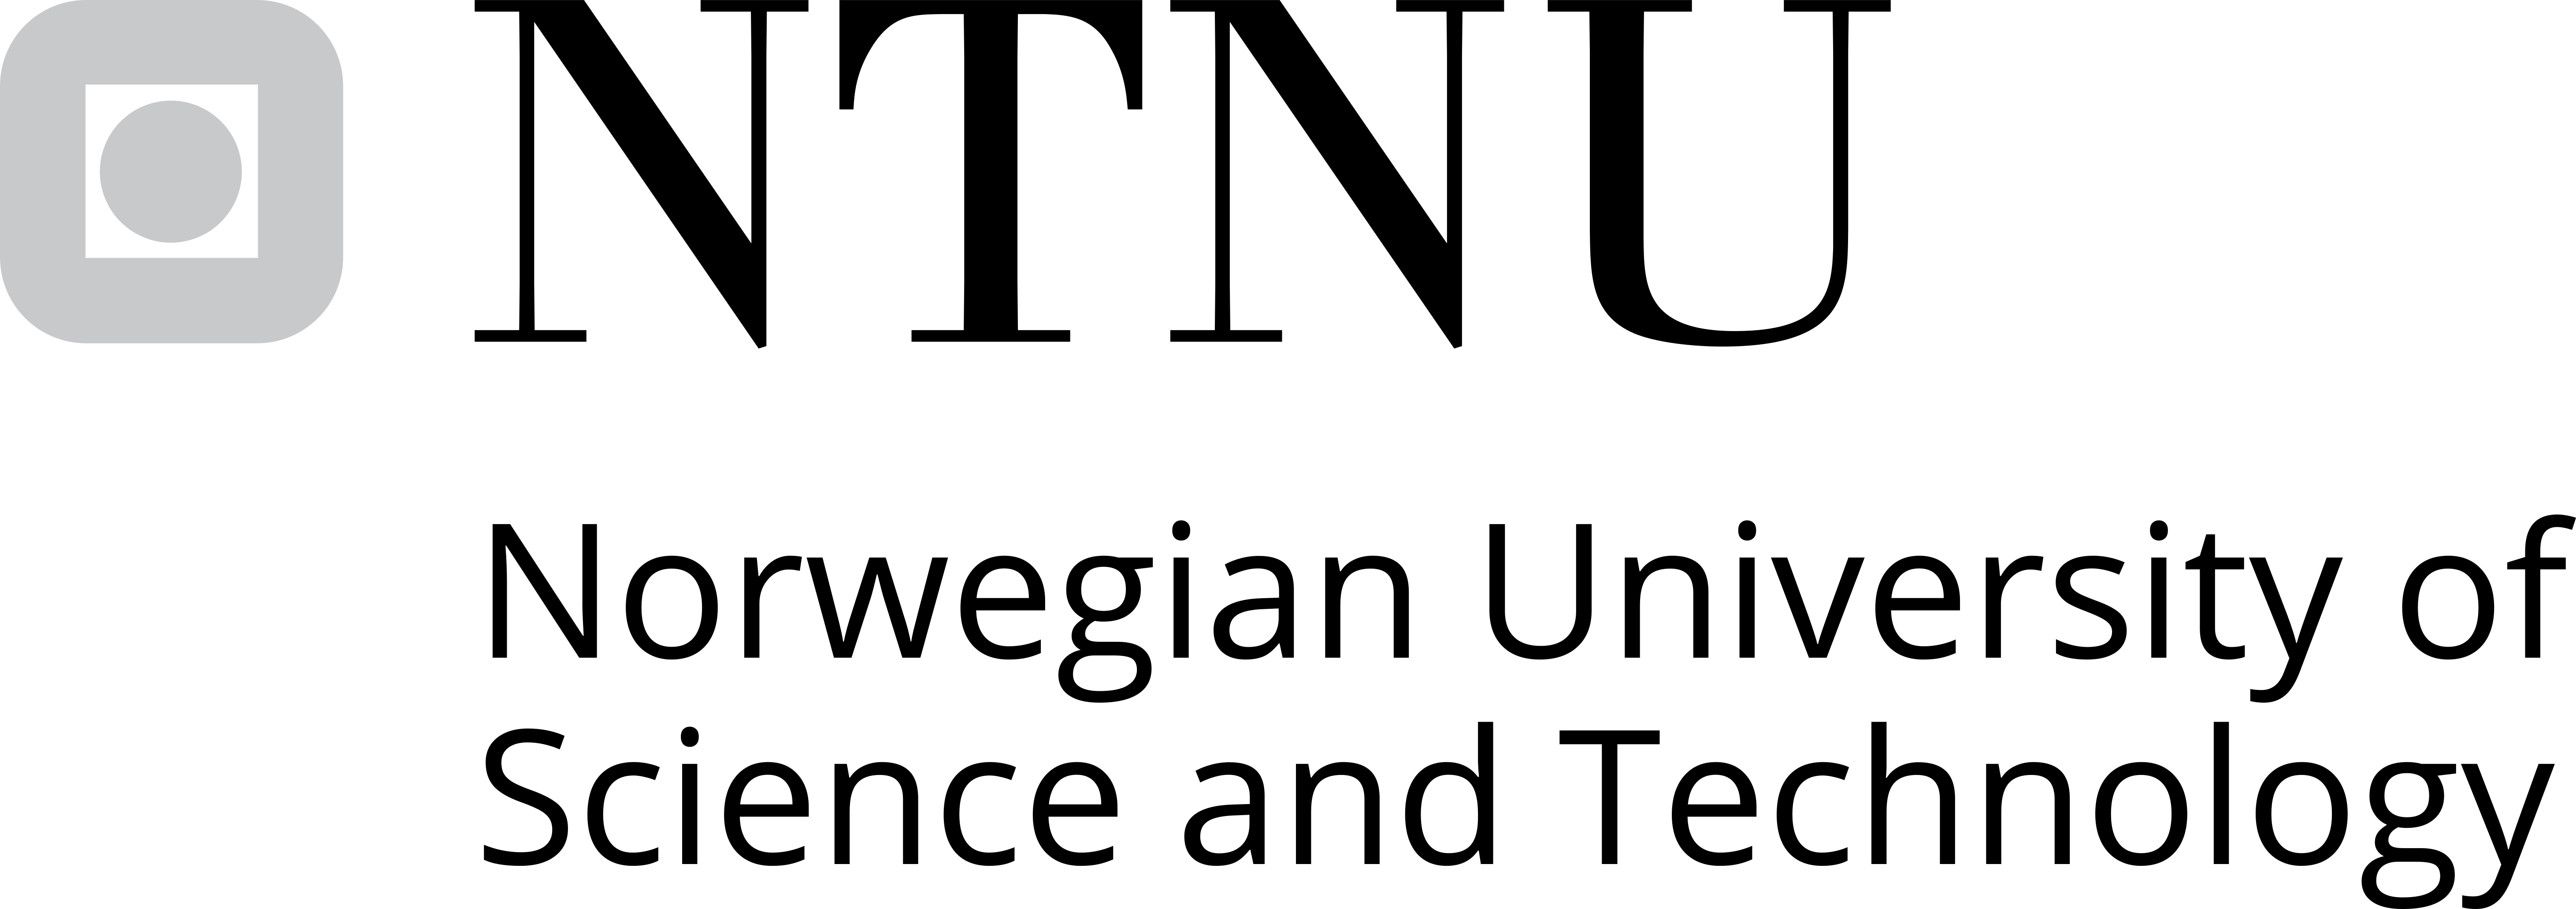
\includegraphics[width=0.39\textwidth]{figures/ntnu-logo-bw.png}

\newpage

% % ============================================================================================================= % %

{
\fontsize{10}{11.4}\selectfont

\noindent \textbf{NTNU} \\
\textit{Norges teknisk-naturvitenskapelige universitet} \\
Norwegian University of Science and Technology \\
\\
Thesis for the Degree of Philosophiae Doctor \\
Faculty of Information Technology and Electrical Engineering \\
Department of Electronic Systems \\
\\
Submitted \hspace{8mm} dd/mm/yyyy; \\
Approved \hspace{8.8mm} dd/mm/yyyy; \\
Date of defense \hspace{1.0mm} dd/mm/yyyy; R{\aa}dsrommet G144 | (time) \\
\\
Supervisors \\
Prof. Supervisor \& Prof. Co-supervisor \\
\\
Assessment Committee
\vspace{-2.0mm}
\begin{itemize}[itemsep=0.7pt, parsep=0.7pt, leftmargin=3.5mm, label=\adforn{43}]
\item 1st opponent \\
Dr. 1st opponent, \\ \textit{Name of the institute in the original language} \\ Name of the institute in English\\ City, Country
\item 2nd opponent \\
Dr. 2nd opponent, \\ \textit{Name of the institute in the original language} \\ Name of the institute in English\\ City, Country
\item Additional members of the committee and administrator \\
Prof. committee
\end{itemize}

\noindent\makebox[\linewidth]{\rule{\paperwidth}{0.4pt}} 

\vspace{3.0mm}

\noindent {\fontsize{8.5}{10}\fontfamily{bch}\selectfont\bfseries\scshape{Title of the Thesis}} \vspace{3.0mm} \\
\noindent Chapters 1-3 \copyright \ 2021 Author (unless otherwise stated) \\
Chapter 4 \copyright \ 2017 Name of journal publisher 1 \\
Chapter 5 \copyright \ 2018 Name of journal publisher 2 \\
Chapter 6 \copyright \ 2020 Name of journal publisher 3 \\
Chapter 7 \copyright \ 2021 Author \\
\\ 
ISBN {123-45-678-9101-2} (printed ver.) \\
ISBN {123-45-678-9101-2} (electronic ver.) \\
ISSN {1234-5678} (printed ver.) \\
ISSN {1234-5678} (online ver.) \\
\\
Doctoral theses at NTNU, 2021:12 \\
\\
Printed by NTNU Grafisk senter
}
%%% Dedication

\pagecolor{abstractback}

\vspace*{3.5cm}

{

\raggedleft \fontfamily{fmm} \selectfont \Large

\color{sophia}

{\large Dedicated to my abc,} \\
Name \\

\vspace{1cm}

{\large And to def,} \\
Name \\

}

\vfill

\clearpage\nopagecolor
\cleardoublepage
%%% Quote

\null\vfill

\null\vfill

\vspace*{\fill}
\parbox{110mm}{

    \lipsum[1]
    \begin{flushright}
        - Some {\fontfamily{bch}\selectfont \scshape One}\par%
    \end{flushright}
    
    \vspace{0.3cm}
    
    \begin{center}
        \pgfornament[scale=0.25,color=sophia]{8}
    \end{center}
    
    \vspace{0.5cm}
    
    \lipsum[2]
    \begin{flushright}
        {\fontfamily{bch}\selectfont \scshape - Someone} \par%
    \end{flushright}

}
\vfill

\vfill

\vfill\vfill

\headerregularsection
%%% Abstract

\chapter*{Abstract}
\addcontentsline{toc}{chapter}{Abstract}

\markboth{Abstract}{Abstract}

\lipsum[1-3] % finalized and formatted on 2021.03.09, checked by me on 2021.03.09
%%% Preface

\chapter*{Preface} 
\addcontentsline{toc}{chapter}{Preface}

\markboth{Preface}%
{Preface}

\lipsum[1-2]

\begin{adjustwidth}{-1mm}{1cm} % 
{\vspace{4mm} \noindent \color{sophia} \small \bfseries \fontfamily{bch} \selectfont \scshape Objectives and Scope} \vspace{5mm}
\end{adjustwidth}

\noindent \lipsum[3-5]

\begin{adjustwidth}{-1mm}{1cm} % 
{\vspace{4mm} \noindent \color{sophia} \small \bfseries \fontfamily{bch} \selectfont \scshape Outlines} \vspace{5mm}
\end{adjustwidth}

\noindent \lipsum[6-8]
\headerregularsection % to neutralize \thispagestyle{empty} from the quote in the last page of PREFACE
%%% Acknowledgement

\chapter*{Acknowledgements}
\addcontentsline{toc}{chapter}{Acknowledgement}

\markboth{Acknowledgements}%
{Acknowledgements}

\lipsum[1-8]

\headerspecialsection % it appears that toc, lof and other pages (e.g. references) generated by book class have a function of "\makeuppercase" within their heading/footer. so to solve this, in practice, it is similar with reference, meaning the same way to tackle this: by issuing "\headerspecialsection"

\cleardoublepage

{
  \hypersetup{linkcolor=sophia} % PREVENTING toc link being colored to "linkcolor" declared in hyperref from preamble, which in this thesis is "ntnu". 

  \cleardoublepage\phantomsection % to fix wrong hyperref
  \pdfbookmark{\contentsname}{toc} % add TOC into the bookmark when it is exported to pdf 
  \tableofcontents
  \label{toc} % used with "Linking the section titles to the ToC, alternative 5"
% %   used with alternative 4, since "part page" linking in this alternative works 
% %   also chapter* can also be recognized, despite its lacking

  \listoffigures\addcontentsline{toc}{chapter}{List of Figures}
  \listoftables\addcontentsline{toc}{chapter}{List of Tables}

  \listoffigures
  \listoftables

}

%%% Nomenclature

\markboth{Nomenclature}{Nomenclature}

\renewcommand{\nompreamble}{
\lipsum[1]
\vspace{1.0em} 
}

%%% in order of alphabet, two columns, line break 
\nomenclature[a]{GaN}{gallium nitride}
\nomenclature[a]{LED}{light-emitting diode}
\nomenclature[a]{AlGaInN}{aluminium gallium \\ indium nitride}
\nomenclature[a]{LDs}{laser diodes}
\nomenclature[a]{InN}{indium nitride}
\nomenclature[a]{AlN}{aluminium nitride}
\nomenclature[a]{UV}{ultraviolet}
\nomenclature[a]{SiC}{silicon carbide}
\nomenclature[a]{Al$_2$O$_3$}{sapphire}
\nomenclature[a]{QCSE}{quantum-confined \\ Stark effect}
\nomenclature[a]{IQE}{internal quantum \\ efficiency}
\nomenclature[a]{HVPE}{hydride-vapor \\ phase epitaxy}
\nomenclature[a]{MBE}{molecular beam epitaxy}
\nomenclature[a]{MOCVD}{metal-organic chemical vapour deposition}
\nomenclature[a]{MOVPE}{metal-organic \\ vapour phase epitaxy}
\nomenclature[a]{GaAsP}{gallium arsenide \\ phosphide}
\nomenclature[a]{AlGaAs}{aluminium gallium \\ arsenide}
\nomenclature[a]{AlGaInP}{aluminium gallium \\ indium phosphide}
\nomenclature[a]{ZnSe}{zinc selenide}
\nomenclature[a]{LEEBI}{low-energy \\ electron-beam \\ irradiation}
\nomenclature[a]{EQE}{external quantum \\ efficiency}
\nomenclature[a]{ITO}{indium tin oxide}
\nomenclature[a]{SEM}{scanning electron \\ microscope}
\nomenclature[a]{RHEED}{reflection high-energy electron diffraction}

\printnomenclature

%=======================================================================
%%% Main matter
\mainmatter

\part{Background}

\chapter[Introduction]{Introduction}
\markboth{Chap. 1\ \ \enspace Introduction}{Chap 1. Introduction}

\regularsection
\headerregularsection

\updatemylof % to be used with "list of figure divider per chapter" (see PREAMBLE)

\begin{sloppypar} % to suppress overfull box

Lorem \index{Lorem} ipsum dolor sit amet, consectetuer adipiscing elit \cite{LIUDIMULYO201767}. Ut purus \index{purus} elit,vestibulum ut, placerat ac, adipiscing vitae, felis \citenum{LIUDIMULYO201767}. Curabitur dictum \index{dictum} gravidamauris. Nam arcu libero, nonummy eget, consectetuer id, vulputate a, magna. Donec vehicula augue eu neque \cite{liudimulyo_2018}. Pellentesque habitant morbi tristique senectuset netus et malesuada fames ac turpis egestas \index{egestas}\citenum{liudimulyo_2018}. Mauris ut leo. Cras viverra metusrhoncus sem \cite{2019liudimulyo}. Nulla et lectus vestibulum urna fringilla ultrices. Phasellus eutellus sit amet tortor gravida placerat \citenum{2019liudimulyo}. Integer sapien est, iaculis in, pretium quis,viverra ac, nunc. Praesent eget sem vel leo ultrices bibendum \cite{liudimulyo2020853}. Aenean faucibus. Morbi dolor nulla, malesuada eu, pulvinar at (\ref{fig:figures/paper-iv/fig-1}), mollis ac, nulla. Curabitur auctorsemper nulla \citenum{liudimulyo2020853}. Donec varius orci eget risus. Duis nibh mi, congue eu, accumsaneleifend, sagittis quis, diam. Duis eget orci sit amet orci dignissim rutrum \cite{LIUDIMULYO201767,liudimulyo_2018,2019liudimulyo,liudimulyo2020853,liudimulyo_unpublished1,liudimulyo_unpublished2}.

\end{sloppypar}

\begin{figure} % \begin{figure} will let LaTeX decide the best figure placement for you ; \begin{figure}[H] for forcing the figure placement here ; in the bottom, \begin{figure}[!b] ; top of the page, \begin{figure}[!t]
    \centering
    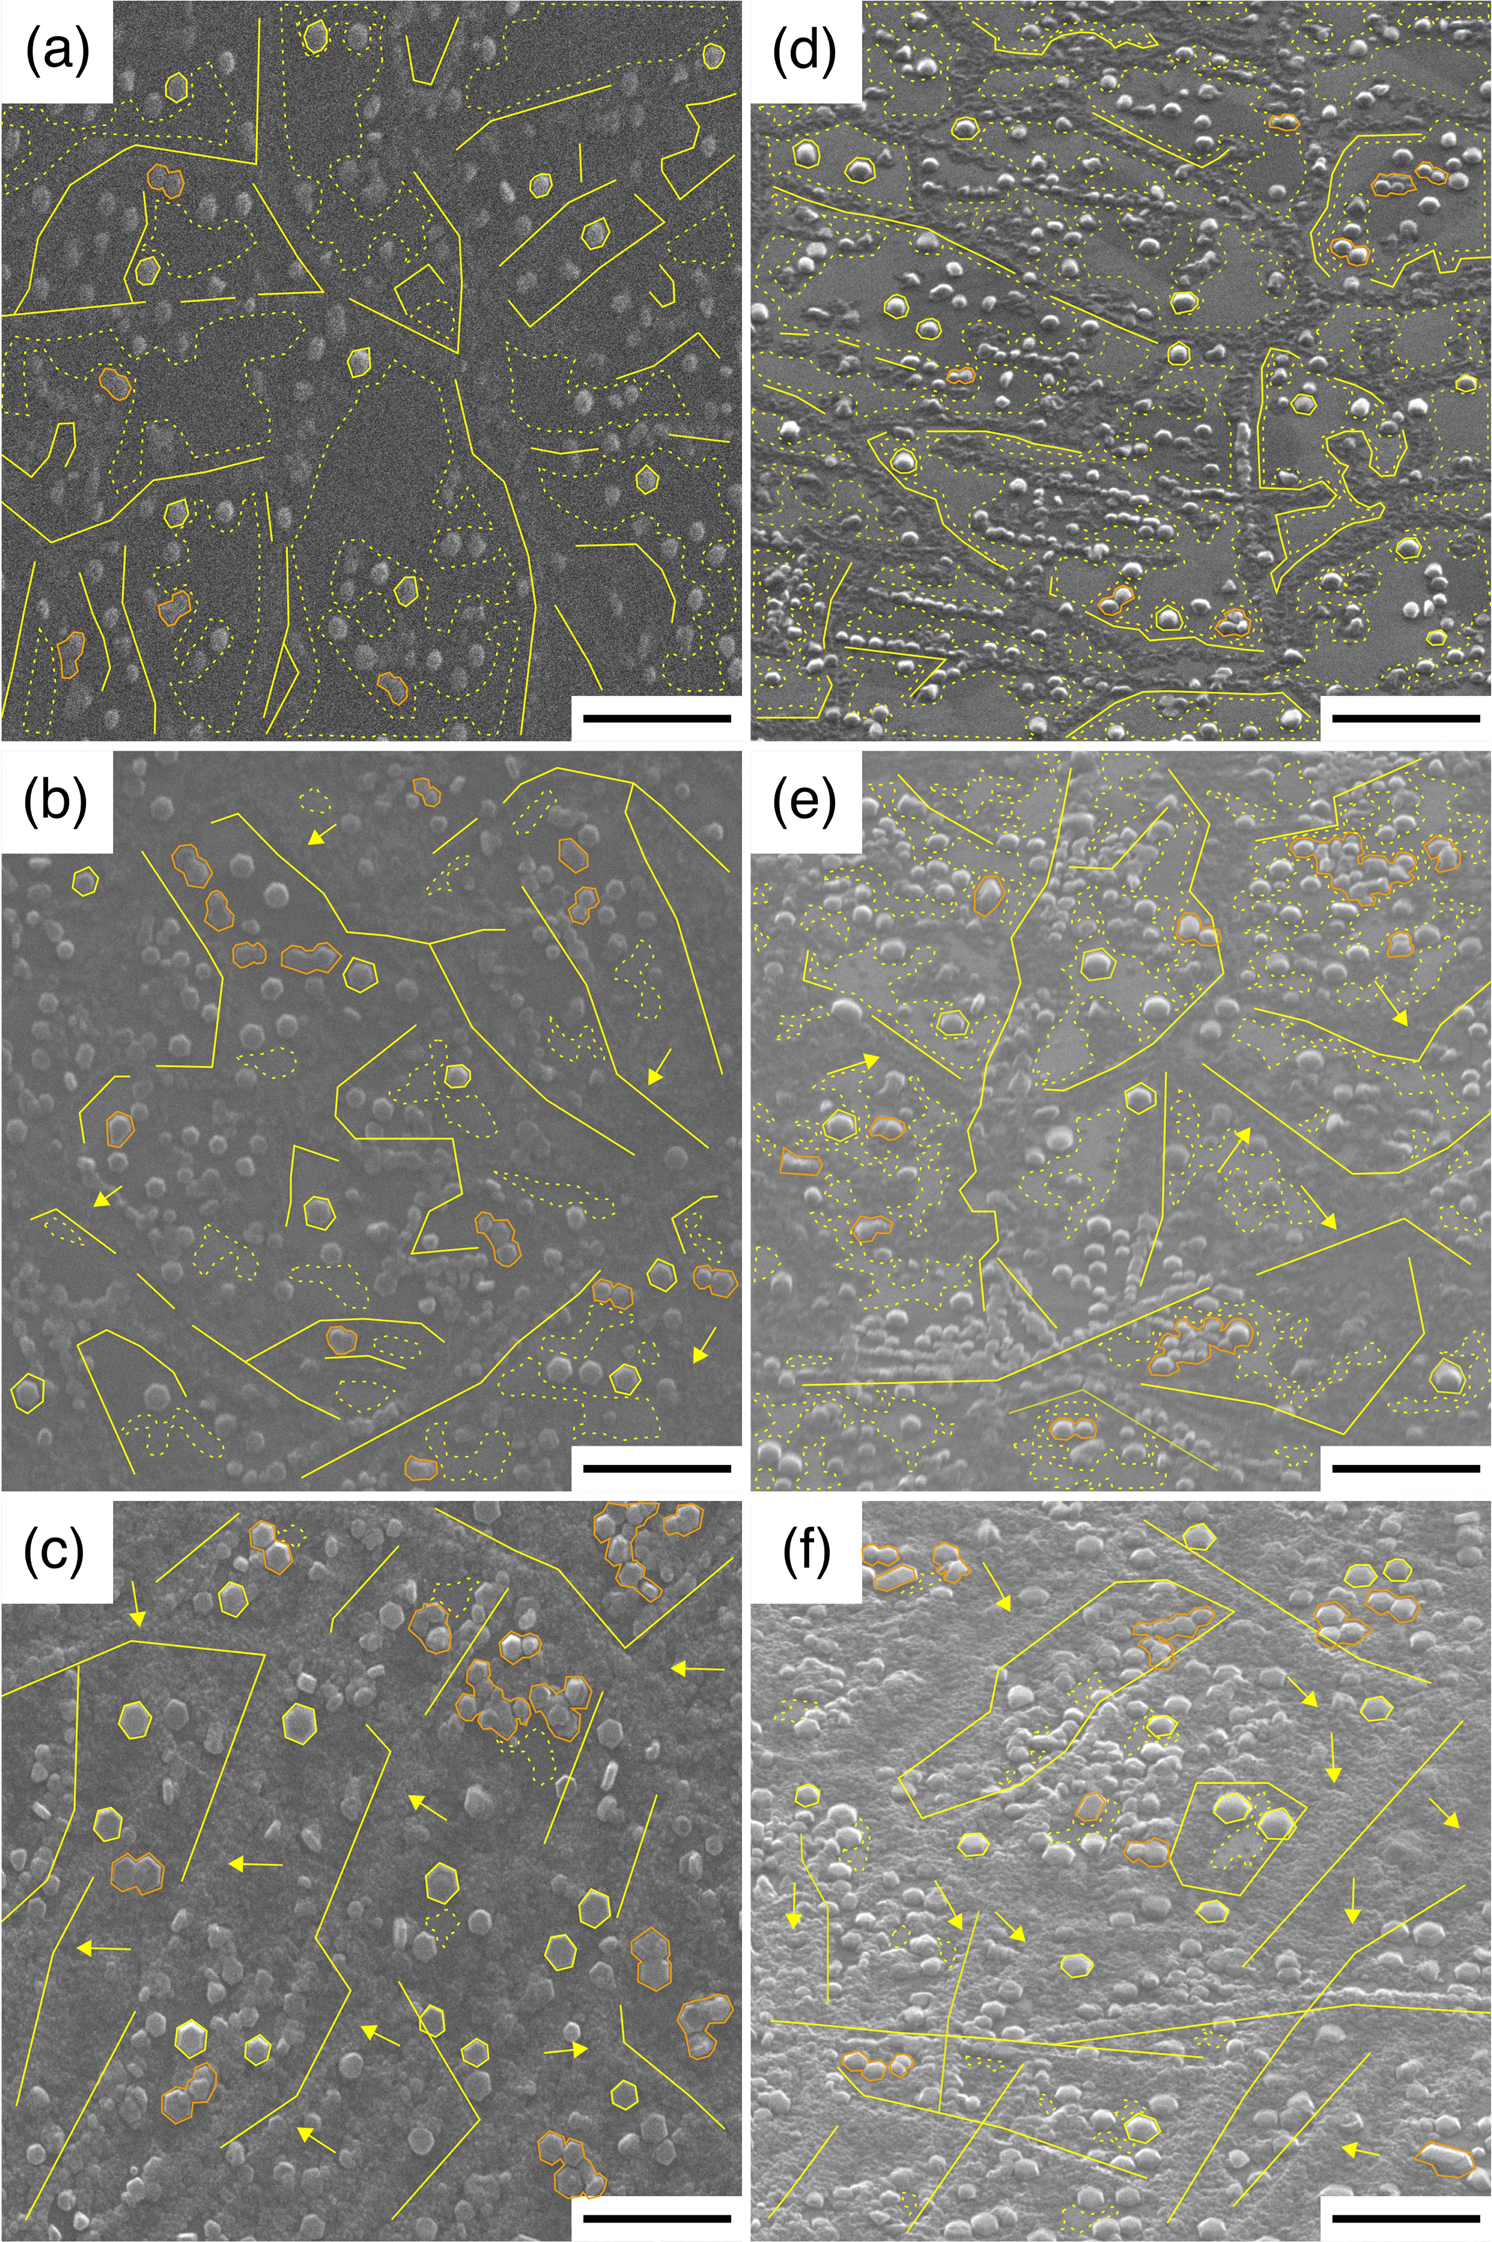
\includegraphics[width=0.95\textwidth]{figures/paper-iv/fig-1.png}
    \caption[SEM images of AlN on graphene formed via different MEE cycles]{SEM images of AlN on graphene formed via different MEE cycles. (\textbf{a},\textbf{d}), (\textbf{b},\textbf{e}) and (\textbf{c},\textbf{f}) are (top-, bird’s eye-view) SEM images of samples A1, A2 and A3, respectively. Scale bars are 1 {\textmu}m. Features marked with yellow lines, yellow (orange) contours and yellow dashed outlines are high-density AlN nanostructures grown along line defects of graphene, individual (coalesced) AlN islands and areas of exposed graphene, respectively. Yellow arrows in samples A2 and A3 show the lateral growth of AlN nanostructures that initially nucleate at the line defects of graphene in sample A1 (adapted with permission from ref. \citenum{liudimulyo2020853} \copyright \ Liudi Mulyo \textit{et al}, 2020.}
    \label{fig:figures/paper-iv/fig-1}
\end{figure}

\section{Section 1 in chapter 1}
\lipsum[2]

\begin{equation}
    EQE = \frac{q \times P_{opt}}{I \times h\nu}
\end{equation}

\lipsum[3-4]

\subsection{Subsection 1.1 of section 1 in chapter 1}
\lipsum[5-7]

\subsection{Subsection 1.2 of section 1 in chapter 1}
\lipsum[8-10]

\clearpage\phantomsection % to fix wrong hyperref to this section
\section[Long section title displayed in the table of content]{Short section title in the chapter}
\sectionmark{Even shorter title on the header}
\lipsum[11-20]

\subsection{Subsection 1.2 of section 2 in chapter 1}
\lipsum[13-14]

%=======================================================================
%%% References 

% \clearpage
\phantomsection
\specialsection % put an indent, see preamble
\headerspecialsection

{\hypersetup{urlcolor=ntnu,linkcolor=sophia} % set clickable URL title color to black, not ntnu like in the main document

\bibliographystyle{unsrtnat-mod}  % NATBIB ref style
\bibliography{references}
}
\chapter[Background]{Background}
\markboth{Chap. 2\ \ \enspace Background}{Chap 2. Background}

\regularsection
\headerregularsection

\updatemylof % to be used with "list of figure divider per chapter" (see PREAMBLE)

\begin{sloppypar} % to suppress overfull box

Lorem \index{Lorem} ipsum dolor sit amet, consectetuer adipiscing elit \cite{LIUDIMULYO201767}. Ut purus \index{purus} elit,vestibulum ut, placerat ac, adipiscing vitae, felis \citenum{LIUDIMULYO201767}. Curabitur dictum \index{dictum} gravidamauris. Nam arcu libero, nonummy eget, consectetuer id, vulputate a, magna. Donec vehicula augue eu neque \cite{liudimulyo_2018}. Pellentesque habitant morbi tristique senectuset netus et malesuada fames ac turpis egestas \index{egestas}\citenum{liudimulyo_2018}. Mauris ut leo. Cras viverra metusrhoncus sem \cite{2019liudimulyo}. Nulla et lectus vestibulum urna fringilla ultrices. Phasellus eutellus sit amet tortor gravida placerat \citenum{2019liudimulyo}. Integer sapien est, iaculis in, pretium quis,viverra ac, nunc. Praesent eget sem vel leo ultrices bibendum \cite{liudimulyo2020853}. Aenean faucibus. Morbi dolor nulla, malesuada eu, pulvinar at (\ref{fig:figures/paper-iv/fig-2}), mollis ac, nulla. Curabitur auctorsemper nulla \citenum{liudimulyo2020853}. Donec varius orci eget risus. Duis nibh mi, congue eu, accumsaneleifend, sagittis quis, diam. Duis eget orci sit amet orci dignissim rutrum \cite{LIUDIMULYO201767,liudimulyo_2018,2019liudimulyo,liudimulyo2020853,liudimulyo_unpublished1,liudimulyo_unpublished2}.

\end{sloppypar}

\begin{figure} % \begin{figure} will let LaTeX decide the best figure placement for you ; \begin{figure}[H] for forcing the figure placement here ; in the bottom, \begin{figure}[!b] ; top of the page, \begin{figure}[!t]
    \centering
    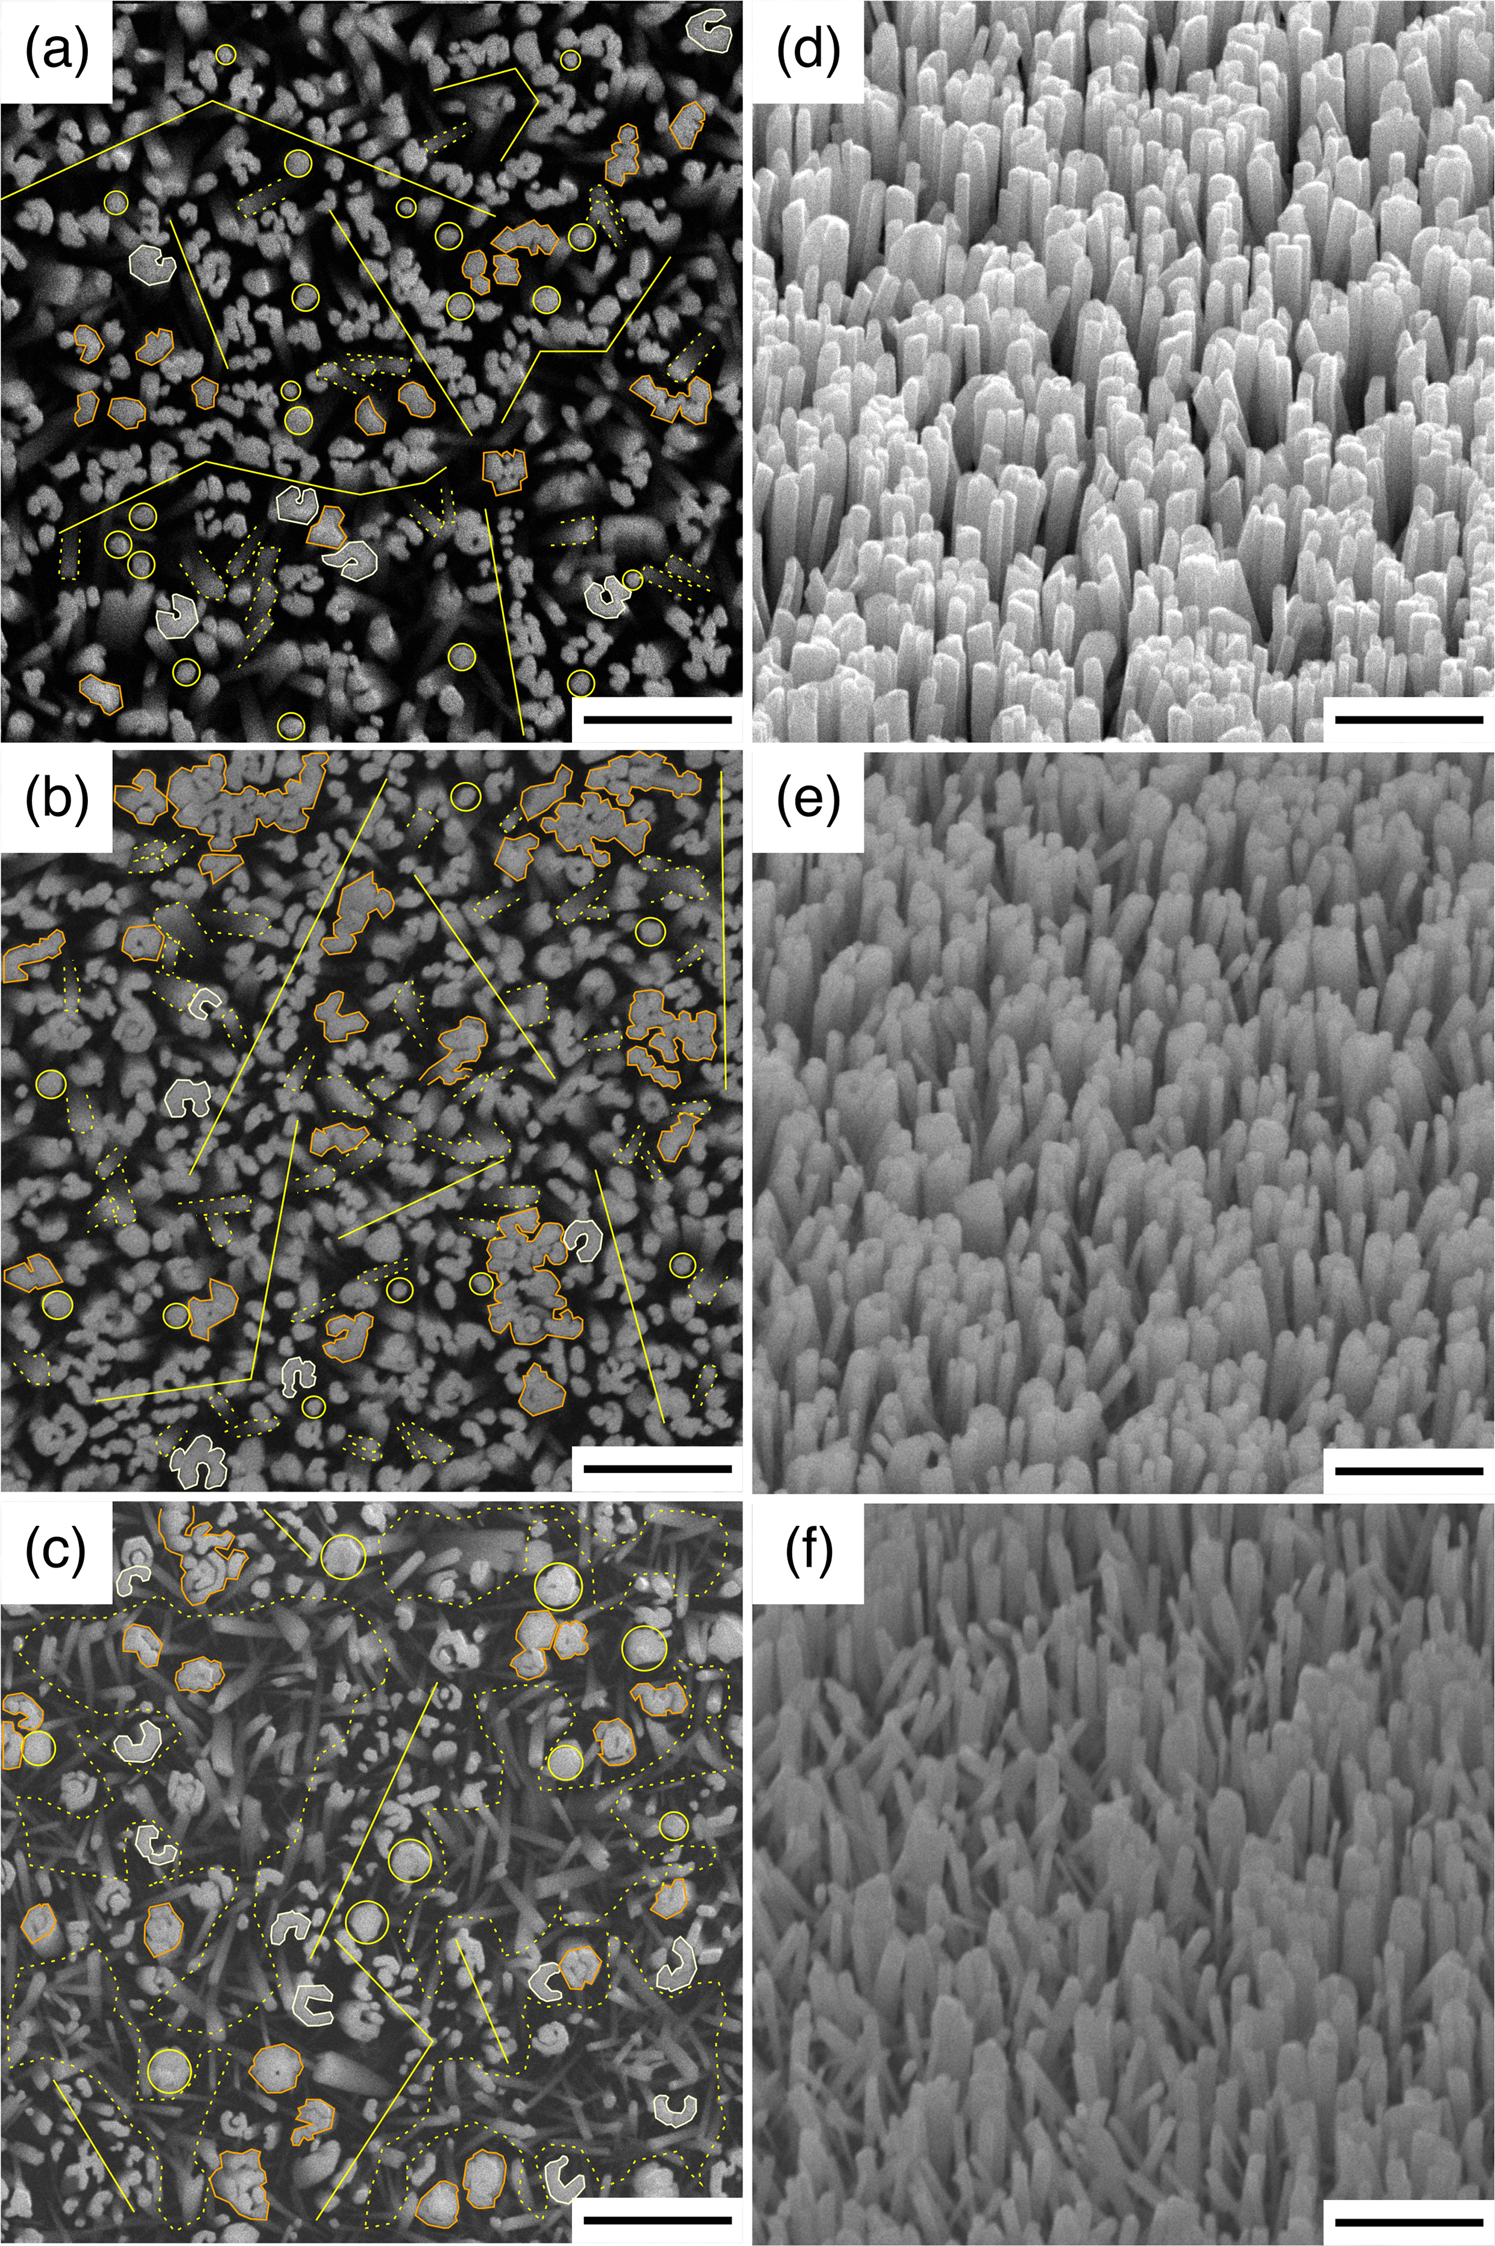
\includegraphics[width=0.95\textwidth]{figures/paper-iv/fig-2.png}
    \caption[SEM images of GaN nanocolumns on graphene formed via different AlN MEE cycles]{SEM images of GaN nanocolumns on graphene formed via different AlN MEE cycles\index{MEE cycles!different AlN}. (\textbf{a},\textbf{d}), (\textbf{b},\textbf{e}) and (\textbf{c},\textbf{f}) are (top-, bird’s eye-view) SEM images of samples G1, G2 and G3, respectively. Scale bars are 1 {\textmu}m. Yellow lines, yellow circles (orange contours) and yellow dashed outlines indicate row of high-density vertical GaN nanocolumns, individual (coalesced) vertical GaN nanocolumns and areas with individual tilted GaN nanocolumns, respectively. White outlines in sample G3 indicate the GaN nanotubular-like structures (adapted with permission from ref. \citenum{liudimulyo2020853} \copyright \ Liudi Mulyo \textit{et al}, 2020.}
    \label{fig:figures/paper-iv/fig-2}
\end{figure}

\section{Section 1 in chapter 2}
\lipsum[2]

\begin{equation}
    EQE = \frac{q \times P_{opt}}{I \times h\nu}
\end{equation}

\lipsum[3-4]

\subsection{Subsection 2.1 of section 1 in chapter 2}
\lipsum[5-7]

\subsection{Subsection 2.2 of section 1 in chapter 2}
\lipsum[8-11]

\clearpage\phantomsection % to fix wrong hyperref to this section
\section[Long section title displayed in the table of content]{Short section title in the chapter}
\sectionmark{Even shorter title on the header}
\lipsum[11-20]

\subsection{Subsection 2.2 of section 2 in chapter 2}
\lipsum[13-14]

%=======================================================================
%%% References 

% \clearpage
\phantomsection
\specialsection % put an indent, see preamble
\headerspecialsection

{\hypersetup{urlcolor=ntnu,linkcolor=sophia} % set clickable URL title color to black, not ntnu like in the main document

\bibliographystyle{unsrtnat-mod}  % NATBIB ref style
\bibliography{references}
}
\chapter[Experimental methods]{Experimental methods}
\markboth{Chap. 3\ \ \enspace Experimental methods}{Chap 2. Experimental methods}

\regularsection
\headerregularsection

\updatemylof % to be used with "list of figure divider per chapter" (see PREAMBLE)
\updatemylot % to be used with "list of table divider per chapter" (see PREAMBLE)

\begin{sloppypar} % to suppress overfull box

Lorem \index{Lorem} ipsum dolor sit amet, consectetuer adipiscing elit \cite{LIUDIMULYO201767}. Ut purus \index{purus} elit,vestibulum ut, placerat ac, adipiscing vitae, felis \citenum{LIUDIMULYO201767}. Curabitur dictum \index{dictum} gravidamauris. Nam arcu libero, nonummy eget, consectetuer id, vulputate a, magna. Donec vehicula augue eu neque \cite{liudimulyo_2018}. Pellentesque habitant morbi tristique senectuset netus et malesuada fames ac turpis egestas \index{egestas}\citenum{liudimulyo_2018}. Mauris ut leo. Cras viverra metusrhoncus sem \cite{2019liudimulyo}. Nulla et lectus vestibulum urna fringilla ultrices. Phasellus eutellus sit amet tortor gravida placerat \citenum{2019liudimulyo}. Integer sapien est, iaculis in, pretium quis,viverra ac, nunc. Praesent eget sem vel leo ultrices bibendum \cite{liudimulyo2020853}. Aenean faucibus. Morbi dolor nulla, malesuada eu, pulvinar at (\ref{fig:figures/paper-iv/fig-3}), mollis ac, nulla. Curabitur auctorsemper nulla \citenum{liudimulyo2020853}. Donec varius orci eget risus. Duis nibh mi, congue eu, accumsaneleifend, sagittis quis, diam. Duis eget orci sit amet orci dignissim rutrum \cite{LIUDIMULYO201767,liudimulyo_2018,2019liudimulyo,liudimulyo2020853,liudimulyo_unpublished1,liudimulyo_unpublished2}.

\end{sloppypar}

\begin{figure}[H] % \begin{figure}[H] for forcing the figure placement here ; in the bottom, \begin{figure}[!b] ; top of the page, \begin{figure}[!t] ; otherwise, \begin{figure} will let LaTeX decide the best figure placement for you
    \centering
    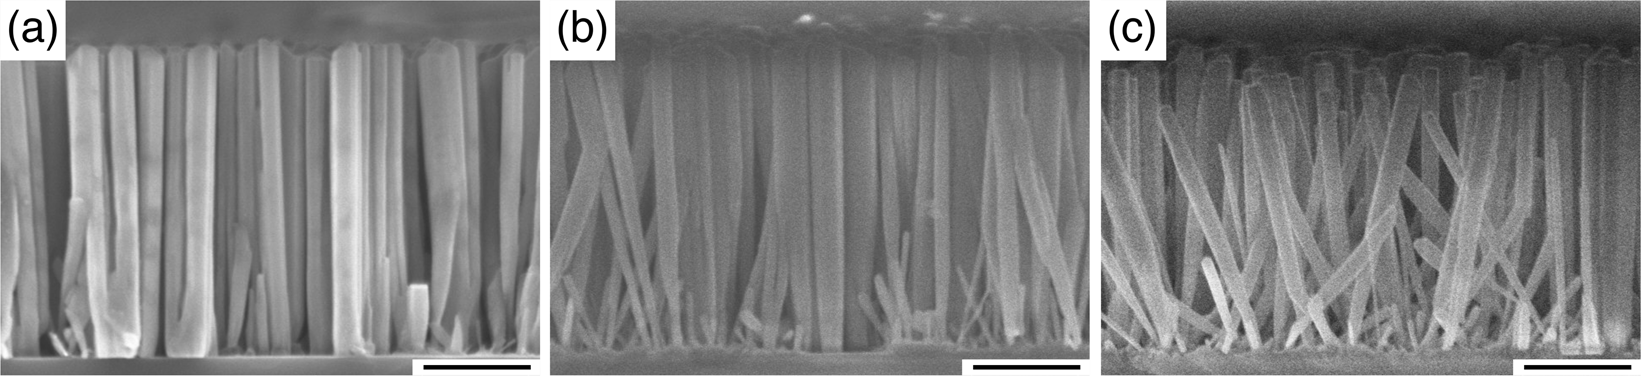
\includegraphics[width=\textwidth]{figures/paper-iv/fig-3.png}
    \caption[Cross-sectional SEM images of GaN nanocolumns on graphene formed via different AlN MEE cycles]{Cross-sectional SEM images of GaN nanocolumns on graphene formed via different AlN MEE cycles. Samples (\textbf{a}) G1, (\textbf{b}) G2, and (\textbf{c}) G3. Scale bars are 500 nm (adapted with permission from ref. \citenum{liudimulyo2020853} \copyright \ Liudi Mulyo \textit{et al}, 2020.}
    \label{fig:figures/paper-iv/fig-3}
\end{figure}

\section{Section 1 in chapter 3}
\lipsum[2]

\begin{equation}
    EQE = \frac{q \times P_{opt}}{I \times h\nu}
\end{equation}

\lipsum[3]
\ref{tab:ch3} lists the experimental conditions of each sample synthesized in this study.

\begin{table}[!h]
\centering
\caption[Experimental conditions described in the ToC]{Experimental conditions.}
\label{tab:ch3}
{\renewcommand{\arraystretch}{1.3}
\begin{tabular}{@{}*{8}{p{.125\textwidth}@{}}}
\toprule
\textbf{Sample ID} & A1    & A2    & A3    & A4    & A5    & A6    & A7    \\
\textbf{T\textsubscript{sub} ($^\circ$C)}  & 100      & 110      & 120      & 130      & 140      & 150      & 160      \\
\textbf{\textPhi\textsubscript{Ga} (Pa)}   & 1.0$\times$10\textsuperscript{-10} & 1.0$\times$10\textsuperscript{-11} & 1.0$\times$10\textsuperscript{-12} & 1.0$\times$10\textsuperscript{-13} & 1.0$\times$10\textsuperscript{-14} & 1.0$\times$10\textsuperscript{-15} & 1.0$\times$10\textsuperscript{-15} \\
\textbf{Q\textsubscript{N} (sccm)} & 1.5     & 1.6     & 1.7     & 1.8     & 1.9     & 2.00     & 2.1 \\
\bottomrule
\end{tabular}
}
\end{table}

\subsection{Subsection 3.1 of section 1 in chapter 3}
\lipsum[5-7]

\subsection{Subsection 3.2 of section 1 in chapter 3}
\lipsum[8-9]

\clearpage\phantomsection % to fix wrong hyperref to this section
\section[Long section title displayed in the table of content]{Short section title in the chapter}
\sectionmark{Even shorter title on the header}
\lipsum[11-20]

\subsection{Subsection 3.2 of section 2 in chapter 3}
\lipsum[13-14]

%=======================================================================
%%% References 

% \clearpage
\phantomsection
\specialsection % put an indent, see preamble
\headerspecialsection

{\hypersetup{urlcolor=ntnu,linkcolor=sophia} % set clickable URL title color to black, not ntnu like in the main document

\bibliographystyle{unsrtnat-mod}  % NATBIB ref style
\bibliography{references}
}

\cleardoublepage\phantomsection % to fix wrong hyperref to \part{Result}
\part{Results}

\chapter[Title of the chapter 4 displayed in the table of contents]
    {Title of the chapter 4 displayed in the page
        \chaptermark{Ch. 4 title in the header}
    }
    \chaptermark{Ch. 4 title in the header}
\label{ch:labelchapter4}

\updatemylof % to be used with "list of figure divider per chapter" (see PREAMBLE)

\regularsection
\headerregularsection

Author 1\textsuperscript{1,\textcolor{sophia}{$\ast$}}, Author 2\textsuperscript{1,2,\textcolor{sophia}{$\ast$}}, Author 3\textsuperscript{3}, Author 4\textsuperscript{1}, Author 5\textsuperscript{1}, Author 6\textsuperscript{1}, Author 7\textsuperscript{2,4,\#} and Author 8\textsuperscript{1,\#} \hfill \textcolor{sophia}{\textsuperscript{$\ast$}\textit{Author 1 and Author 2 contributed equally to this study.}} \newline

\let\thefootnote\relax\footnotetext{\textsuperscript{1}Department X, University 1, City A, Country B. 
\textsuperscript{2}Department Y, University 2, City C, Country D. 
\textsuperscript{3}Institute E, City F, Country G. 
\textsuperscript{4}Research Center H, University I, City J, Country K. 
\textsuperscript{\#}e-mail: \href{mailto:author7@university2.ac.countryD}{author7@university2.ac.countryD} and \href{mailto:author8@universityI.countryK}{author8@universityI.countryK}}

\noindent First published in: \textit{Scientific Reports} \textbf{10}, 853 (2020). \hfill \break
DOI: \href{https://doi.org/10.1038/s41598-019-55424-z}{10.1038/s41598-019-55424-z} 

\begin{wrapfigure}[3]{l}{0.2\textwidth}
    
\includegraphics[width=0.2\textwidth]{figures/by.png}
\end{wrapfigure} 

\noindent \textcolor{white}{test} \newline \textbf{Open Access} This article is licensed under a Creative Commons Attribution 4.0 International License. It means that unrestricted use, sharing, adaptation, distribution, and reproduction in any medium or format are allowed, as long as the original author(s) and the source are appropriately credited, a link to the Creative Commons license is provided, and any changes made are indicated. To view a copy of this license, please visit \href{http://creativecommons.org/licenses/by/4.0/}{http://creativecommons.org/licenses/by/4.0/}. \newline

\noindent \copyright \ Liudi Mulyo \textit{et al}, 2020. \newline

\noindent \textbf{Contributions} \newline
\noindent \lipsum[2]

%%%%%%%%%%%%%%%%%%%%%%%%%%%%%%%%%%%%%%%%%%%%%%%%%%%%%%%%%%%%%%%%%%%%%%%%%%%%%%%%%%%%%%%%%%%%%%%%%%%%%%%%%%%%%%%%%%%%%%%%%%%

\tcbset{enhanced,colback=abstractback,colframe=sophia,fonttitle=\bfseries}
\begin{tcolorbox}[left=3.35cm,grow to left by=3.5cm,right=3.33cm,grow to right by=3.5cm,title={\normalfont \color{White} \small \fontfamily{bch} \selectfont \scshape Abstract}]
% https://tex.stackexchange.com/questions/232878/inserting-pictures-in-tcolorbox
% https://tex.stackexchange.com/questions/169794/outer-margin-of-tcolorbox/169877
% https://tex.stackexchange.com/questions/11484/how-to-draw-a-frame-box-around-an-arbitrary-large-piece-of-text-figures-whatever
\begin{minipage}[t]{\linewidth}
\vspace*{-29pt}
\phantomsection % to fix wrong hyperref to "Abstract" 
\section*{} % for linking from TOC (only one way)
\addcontentsline{toc}{section}{Abstract}
\begin{sloppypar}
\lipsum[1]
\end{sloppypar}

\end{minipage}

\vspace*{3.5pt}
\end{tcolorbox}

%%%%%%%%%%%%%%%%%%%%%%%%%%%%%%%%%%%%%%%%%%%%%%%%%%%%%%%%%%%%%%%%%%%%%%%%%%%%%%%%%%%%%%%%%%%%%%%%%%%%%%%%%%%%%%%%%%%%%%%%%%%

\begin{sloppypar} % to suppress overfull box

Lorem \index{Lorem} ipsum dolor sit amet, consectetuer adipiscing elit \cite{LIUDIMULYO201767}. Ut purus \index{purus} elit,vestibulum ut, placerat ac, adipiscing vitae, felis \citenum{LIUDIMULYO201767}. Curabitur dictum \index{dictum} gravidamauris. Nam arcu libero, nonummy eget, consectetuer id, vulputate a, magna. Donec vehicula augue eu neque \cite{liudimulyo_2018}. Pellentesque habitant morbi tristique senectuset netus et malesuada fames ac turpis egestas \index{egestas}\citenum{liudimulyo_2018}. Mauris ut leo. Cras viverra metusrhoncus sem \cite{2019liudimulyo}. Nulla et lectus vestibulum urna fringilla ultrices. Phasellus eutellus sit amet tortor gravida placerat \citenum{2019liudimulyo}. Integer sapien est, iaculis in, pretium quis,viverra ac, nunc. Praesent eget sem vel leo ultrices bibendum \cite{liudimulyo2020853}. Aenean faucibus. Morbi dolor nulla, malesuada eu, pulvinar at (\ref{fig:figures/paper-iv/fig-4}), mollis ac, nulla. Curabitur auctorsemper nulla \citenum{liudimulyo2020853}. Donec varius orci eget risus. Duis nibh mi, congue eu, accumsaneleifend, sagittis quis, diam. Duis eget orci sit amet orci dignissim rutrum \cite{LIUDIMULYO201767,liudimulyo_2018,2019liudimulyo,liudimulyo2020853,liudimulyo_unpublished1,liudimulyo_unpublished2}. For more information, see \hyperref[appendix:A]{Appendix A}, specifically in \ref{tab:appendixA}.

\end{sloppypar}

\begin{figure} % \begin{figure} will let LaTeX decide the best figure placement for you ; \begin{figure}[H] for forcing the figure placement here ; in the bottom, \begin{figure}[!b] ; top of the page, \begin{figure}[!t]
    \centering
    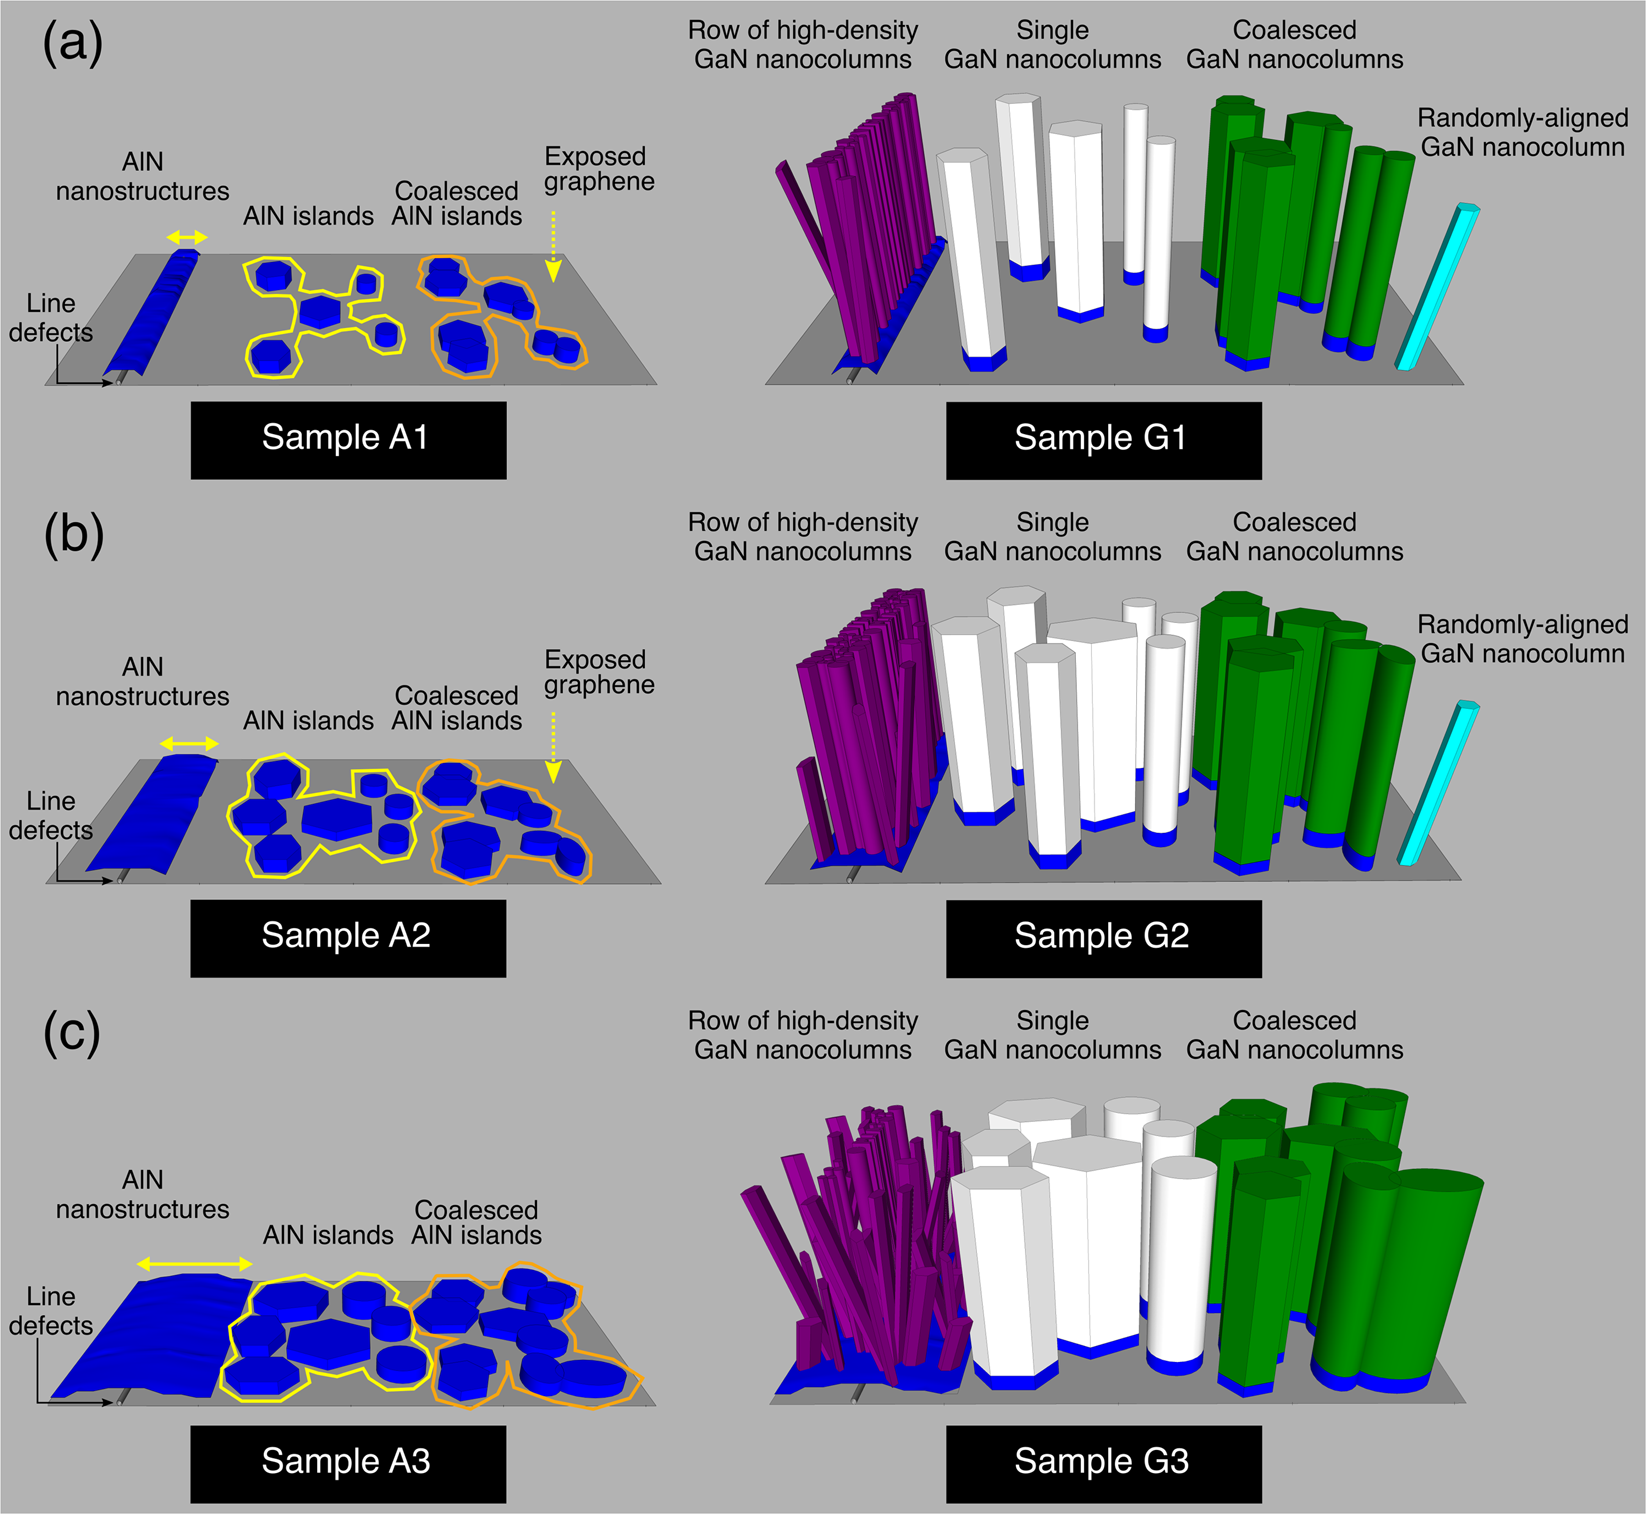
\includegraphics[width=\textwidth]{figures/paper-iv/fig-4.png}
    \caption[Simplified schematics of the AlN buffer structures and GaN nanocolumn formation on graphene]{Simplified schematics of the AlN buffer structures and GaN nanocolumn formation on graphene. Samples (\textbf{a}) A1-G1, (\textbf{b}) A2-G2 and (\textbf{c}) A3-G3. There are two possible AlN (blue) nanostructures forming on graphene: 1) AlN islands and 2) AlN nanostructures along the line defects of graphene (the yellow arrows indicate their lateral growth spread further away from the line defects). Single (white) and coalesced (green) vertical GaN nanocolumn structures are nucleated from the AlN islands, while row of high-density nanocolumns (purple) form on the AlN nanostructures that spread from the line defects. Additional tilted nanocolumns (cyan) are likely to grow on exposed graphene (adapted with permission from ref. \citenum{liudimulyo2020853} \copyright \ Liudi Mulyo \textit{et al}, 2020.}
    \label{fig:figures/paper-iv/fig-4}
\end{figure}

\section{Section 1 in chapter 4}
\lipsum[2-4]

\subsection{Subsection 4.1 of section 1 in chapter 4}
\lipsum[5-7]

\subsection{Subsection 4.2 of section 1 in chapter 4}
\lipsum[8-11]

\clearpage\phantomsection % to fix wrong hyperref to this section
\section[Long section title displayed in the table of content]{Short section title in the chapter}
\sectionmark{Even shorter title on the header}
\lipsum[11-20]

\subsection{Subsection 4.2 of section 2 in chapter 4}
\lipsum[13-14]

%=======================================================================
%%% References 

% \clearpage
\phantomsection
\specialsection % put an indent, see preamble
\headerspecialsection

{\hypersetup{urlcolor=ntnu,linkcolor=sophia} % set clickable URL title color to black, not ntnu like in the main document

\bibliographystyle{unsrtnat-mod}  % NATBIB ref style
\bibliography{references}
}
\chapter[Title of the chapter 5 displayed \\ in the table of contents]
    {Title of the chapter 5 displayed in the page
        \chaptermark{Ch. 5 title in the header}
    }
    \chaptermark{Ch. 5 title in the header}
\label{ch:labelchapter5}

\updatemylof % to be used with "list of figure divider per chapter" (see PREAMBLE)
\updatemylot % to be used with "list of table divider per chapter" (see PREAMBLE)

\regularsection
\headerregularsection

Author 1\textsuperscript{1,\textcolor{sophia}{$\ast$}}, Author 2\textsuperscript{1,2,\textcolor{sophia}{$\ast$}}, Author 3\textsuperscript{3}, Author 4\textsuperscript{1}, Author 5\textsuperscript{1}, Author 6\textsuperscript{1}, Author 7\textsuperscript{2,4,\#} and Author 8\textsuperscript{1,\#} \hfill  \newline

\let\thefootnote\relax\footnotetext{\textsuperscript{1}Department X, University 1, City A, Country B. 
\textsuperscript{2}Department Y, University 2, City C, Country D. 
\textsuperscript{3}Institute E, City F, Country G. 
\textsuperscript{4}Research Center H, University I, City J, Country K. 
\textsuperscript{\#}e-mail: \href{mailto:author7@university2.ac.countryD}{author7@university2.ac.countryD} and \href{mailto:author8@universityI.countryK}{author8@universityI.countryK}}

\noindent First published in: \textit{Scientific Reports} \textbf{10}, 853 (2020). \hfill \break
DOI: \href{https://doi.org/10.1038/s41598-019-55424-z}{10.1038/s41598-019-55424-z} 

\begin{wrapfigure}[3]{l}{0.2\textwidth}
    
\includegraphics[width=0.2\textwidth]{figures/by.png}
\end{wrapfigure} 

\noindent \textcolor{white}{test} \newline \textbf{Open Access} This article is licensed under a Creative Commons Attribution 4.0 International License. It means that unrestricted use, sharing, adaptation, distribution, and reproduction in any medium or format are allowed, as long as the original author(s) and the source are appropriately credited, a link to the Creative Commons license is provided, and any changes made are indicated. To view a copy of this license, please visit \href{http://creativecommons.org/licenses/by/4.0/}{http://creativecommons.org/licenses/by/4.0/}. \newline

\noindent \copyright \ Liudi Mulyo \textit{et al}, 2020. \newline

\noindent \textbf{Contributions} \newline
\noindent \lipsum[2]

%%%%%%%%%%%%%%%%%%%%%%%%%%%%%%%%%%%%%%%%%%%%%%%%%%%%%%%%%%%%%%%%%%%%%%%%%%%%%%%%%%%%%%%%%%%%%%%%%%%%%%%%%%%%%%%%%%%%%%%%%%%

\tcbset{enhanced,colback=abstractback,colframe=sophia,fonttitle=\bfseries}
\begin{tcolorbox}[left=3.35cm,grow to left by=3.5cm,right=3.33cm,grow to right by=3.5cm,title={\normalfont \color{White} \small \fontfamily{bch} \selectfont \scshape Abstract}]
% https://tex.stackexchange.com/questions/232878/inserting-pictures-in-tcolorbox
% https://tex.stackexchange.com/questions/169794/outer-margin-of-tcolorbox/169877
% https://tex.stackexchange.com/questions/11484/how-to-draw-a-frame-box-around-an-arbitrary-large-piece-of-text-figures-whatever
\begin{minipage}[t]{\linewidth}
\vspace*{-29pt}
\phantomsection % to fix wrong hyperref to "Abstract" 
\section*{} % for linking from TOC (only one way)
\addcontentsline{toc}{section}{Abstract}
\begin{sloppypar}
\lipsum[1]
\end{sloppypar}

\end{minipage}

\vspace*{3.5pt}
\end{tcolorbox}

%%%%%%%%%%%%%%%%%%%%%%%%%%%%%%%%%%%%%%%%%%%%%%%%%%%%%%%%%%%%%%%%%%%%%%%%%%%%%%%%%%%%%%%%%%%%%%%%%%%%%%%%%%%%%%%%%%%%%%%%%%%

\begin{sloppypar} % to suppress overfull box

As in \Autoref{ch:labelchapter4}. Lorem \index{Lorem} ipsum dolor sit amet, consectetuer adipiscing elit \cite{LIUDIMULYO201767}. Ut purus \index{purus} elit,vestibulum ut, placerat ac, adipiscing vitae, felis \citenum{LIUDIMULYO201767}. Curabitur dictum \index{dictum} gravidamauris. Nam arcu libero, nonummy eget, consectetuer id, vulputate a, magna. Donec vehicula augue eu neque \cite{liudimulyo_2018}. Pellentesque habitant morbi tristique senectuset netus et malesuada fames ac turpis egestas \index{egestas}\citenum{liudimulyo_2018}. Mauris ut leo. Cras viverra metusrhoncus sem \cite{2019liudimulyo}. Nulla et lectus vestibulum urna fringilla ultrices. Phasellus eutellus sit amet tortor gravida placerat \citenum{2019liudimulyo}. Integer sapien est, iaculis in, pretium quis,viverra ac, nunc. Praesent eget sem vel leo ultrices bibendum \cite{liudimulyo2020853}. Aenean faucibus. Morbi dolor nulla, malesuada eu, pulvinar at (\ref{fig:figures/paper-iv/fig-5}), mollis ac, nulla. Curabitur auctorsemper nulla \citenum{liudimulyo2020853}. Donec varius orci eget risus. Duis nibh mi, congue eu, accumsaneleifend, sagittis quis, diam. Duis eget orci sit amet orci dignissim rutrum \cite{LIUDIMULYO201767,liudimulyo_2018,2019liudimulyo,liudimulyo2020853,liudimulyo_unpublished1,liudimulyo_unpublished2}. For more information, see \hyperref[appendix:B]{Appendix B}, specifically in \ref{tab:appendixB}.

\end{sloppypar}

\begin{figure} % \begin{figure} will let LaTeX decide the best figure placement for you ; \begin{figure}[H] for forcing the figure placement here ; in the bottom, \begin{figure}[!b] ; top of the page, \begin{figure}[!t]
    \centering
    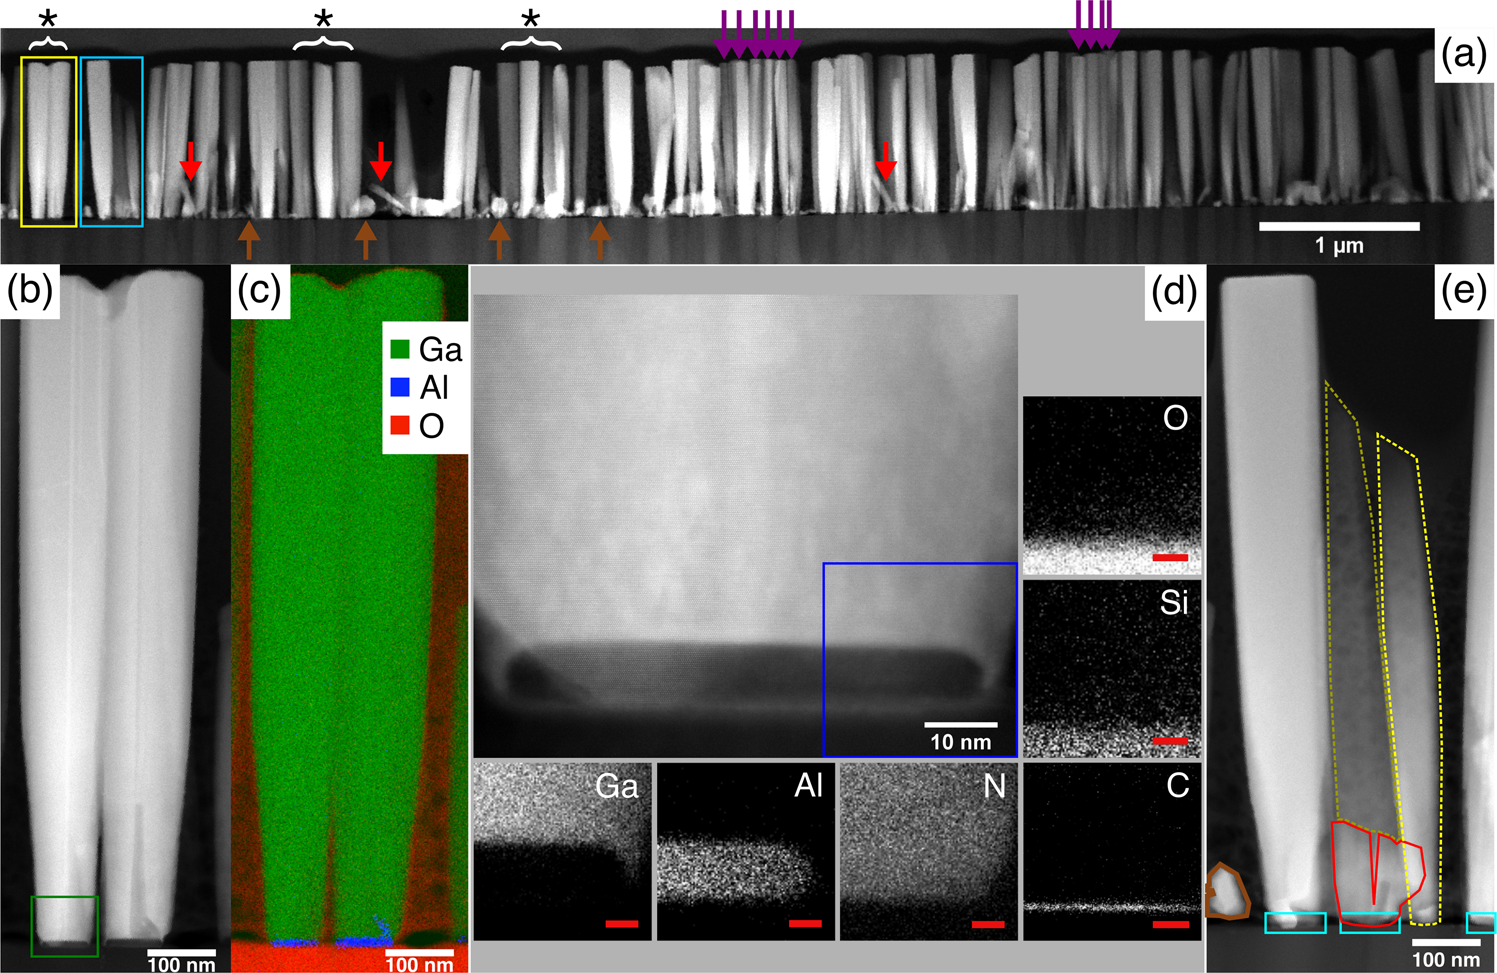
\includegraphics[width=\textwidth]{figures/paper-iv/fig-5.png}
    \caption[TEM image of GaN nanocolumn sample synthesized with\newline nominally the same growth conditions as sample G1]{TEM image of GaN nanocolumn sample synthesized with nominally the same growth conditions as sample G1. (\textbf{a}) Overview cross-sectional HAADF STEM image, showing vertical GaN nanocolumns (star-marked and purple arrows), inclined GaN nanocolumns (red arrows) and GaN crystallites (brown arrows). (\textbf{b}) HAADF STEM image of two GaN nanocolumns within yellow frame in \textbf{a}. (\textbf{c}) Combined color map of the Ga (green), Al (blue) and O (red) elemental distributions (EDS/EELS) on the corresponding region in \textbf{b}. (\textbf{d}) Magnified image of the lower part of the GaN nanocolumn near the interface of the left GaN nanocolumn in \textbf{b} (green frame), with the elemental mapping near the interfaces between the GaN nanocolumn, AlN island, graphene and silica glass (blue frame) by EDS (Ga, Al, Si) and EELS (N, O, C). The red scale bars are 5 nm. (\textbf{e}) HAADF STEM image of the GaN nanocolumns that is light-blue framed in \textbf{a}. The inclined GaN nanocolumn (yellow-dashed line) is possibly directly nucleated on graphene (indicated by the absence of any AlN layer [cyan frames] at the base). There are two broken GaN nanocolumns (red framed area) sharing the same AlN island and another inclined GaN nanocolumn (dark-yellow dashed line) in the background. An irregular GaN crystallite (brown outline) likely grown directly on graphene is also observed (adapted with permission from ref. \citenum{liudimulyo2020853} \copyright \ Liudi Mulyo \textit{et al}, 2020.}
    \label{fig:figures/paper-iv/fig-5}
\end{figure}

\section{Section 1 in chapter 5}
\lipsum[2-4]

\subsection{Subsection 5.1 of section 1 in chapter 5}
\lipsum[5-7]

\subsection{Subsection 5.2 of section 1 in chapter 5}
\lipsum[8-11]

\clearpage\phantomsection % to fix wrong hyperref to this section
\section[Long section title displayed in the table of content]{Short section title in the chapter}
\sectionmark{Even shorter title on the header}
\lipsum[11-18]
See \ref{tab:ch5}

\begin{table}[!h]
\centering
\caption{Micro-Raman peak positions, intensities and ratios}
\label{tab:ch5}
{\fontsize{7}{6}\selectfont
{\renewcommand{\arraystretch}{2}
\begin{tabular}{cccccccc}
\toprule
\multirow{3}{*}{\textbf{Sample}} & 
\multirow{3}{*}{\textbf{\begin{tabular}[c]{@{}c@{}}Median\\ D/G ratio\end{tabular}}} & 
\multicolumn{2}{c}{\textbf{Median G}} & 
\multicolumn{3}{c}{\textbf{Median 2D}} & 
\multirow{3}{*}{\textbf{\begin{tabular}[c]{@{}c@{}}Median \\ 2D/G ratio\end{tabular}}} \\
\cmidrule(l){3-4} \cmidrule(l){3-4} \cmidrule(l){3-4} \cmidrule(l){5-7} \cmidrule(l){5-7} \cmidrule(l){5-7} % repeated three times to increase the line thickness
  &  & \textbf{\begin{tabular}[c]{@{}c@{}}Position \\ {[} cm\textsuperscript{-1} {]}\end{tabular}} & \textbf{\begin{tabular}[c]{@{}c@{}}Intensity \\ {[} cps {]}\end{tabular}} & \textbf{\begin{tabular}[c]{@{}c@{}}Position \\ {[} cm\textsuperscript{-1} {]}\end{tabular}} & \textbf{\begin{tabular}[c]{@{}c@{}}Intensity \\ {[} cps {]}\end{tabular}} & \textbf{\begin{tabular}[c]{@{}c@{}}FWHM \\ {[} cm\textsuperscript{-1} {]}\end{tabular}} &  \\
\midrule
\begin{tabular}[c]{@{}c@{}}DLG before\\ MBE growth\end{tabular} & 1 & 2 & 3 & 4 & 5 & 6 & 7 \\
\rowcolor{Gray} \begin{tabular}[c]{@{}c@{}}DLG after\\ MBE growth\end{tabular} & 1 & 2 & 3 & 4 & 5 & 6 & 7 \\
\bottomrule
\end{tabular}
}
}
\end{table}

\subsection{Subsection 5.2 of section 2 in chapter 5}
\lipsum[13-14]

%=======================================================================
%%% References 

% \clearpage
\phantomsection
\specialsection % put an indent, see preamble
\headerspecialsection

{\hypersetup{urlcolor=ntnu,linkcolor=sophia} % set clickable URL title color to black, not ntnu like in the main document

\bibliographystyle{unsrtnat-mod}  % NATBIB ref style
\bibliography{references}
}
\chapter[Title of the chapter 6 displayed in the table of contents]
    {Title of the chapter 6 displayed in the page
        \chaptermark{Ch. 6 title in the header}
    }
    \chaptermark{Ch. 6 title in the header}
\label{ch:labelchapter6}

\updatemylof % to be used with "list of figure divider per chapter" (see PREAMBLE)
\updatemylot % to be used with "list of table divider per chapter" (see PREAMBLE)

\regularsection
\headerregularsection

Author 1\textsuperscript{1,\textcolor{sophia}{$\ast$}}, Author 2\textsuperscript{1,2,\textcolor{sophia}{$\ast$}}, Author 3\textsuperscript{3}, Author 4\textsuperscript{1}, Author 5\textsuperscript{1}, Author 6\textsuperscript{1}, Author 7\textsuperscript{2,4,\#} and Author 8\textsuperscript{1,\#} \hfill  \newline

\let\thefootnote\relax\footnotetext{\textsuperscript{1}Department X, University 1, City A, Country B. 
\textsuperscript{2}Department Y, University 2, City C, Country D. 
\textsuperscript{3}Institute E, City F, Country G. 
\textsuperscript{4}Research Center H, University I, City J, Country K. 
\textsuperscript{\#}e-mail: \href{mailto:author7@university2.ac.countryD}{author7@university2.ac.countryD} and \href{mailto:author8@universityI.countryK}{author8@universityI.countryK}}

\noindent First published in: \textit{Scientific Reports} \textbf{10}, 853 (2020). \hfill \break
DOI: \href{https://doi.org/10.1038/s41598-019-55424-z}{10.1038/s41598-019-55424-z} 

\begin{wrapfigure}[3]{l}{0.2\textwidth}
    
\includegraphics[width=0.2\textwidth]{figures/by.png}
\end{wrapfigure} 

\noindent \textcolor{white}{test} \newline \textbf{Open Access} This article is licensed under a Creative Commons Attribution 4.0 International License. It means that unrestricted use, sharing, adaptation, distribution, and reproduction in any medium or format are allowed, as long as the original author(s) and the source are appropriately credited, a link to the Creative Commons license is provided, and any changes made are indicated. To view a copy of this license, please visit \href{http://creativecommons.org/licenses/by/4.0/}{http://creativecommons.org/licenses/by/4.0/}. \newline

\noindent \copyright \ Liudi Mulyo \textit{et al}, 2020. \newline

\noindent \textbf{Contributions} \newline
\noindent \lipsum[2]

%%%%%%%%%%%%%%%%%%%%%%%%%%%%%%%%%%%%%%%%%%%%%%%%%%%%%%%%%%%%%%%%%%%%%%%%%%%%%%%%%%%%%%%%%%%%%%%%%%%%%%%%%%%%%%%%%%%%%%%%%%%

\tcbset{enhanced,colback=abstractback,colframe=sophia,fonttitle=\bfseries}
\begin{tcolorbox}[left=3.35cm,grow to left by=3.5cm,right=3.33cm,grow to right by=3.5cm,title={\normalfont \color{White} \small \fontfamily{bch} \selectfont \scshape Abstract}]
% https://tex.stackexchange.com/questions/232878/inserting-pictures-in-tcolorbox
% https://tex.stackexchange.com/questions/169794/outer-margin-of-tcolorbox/169877
% https://tex.stackexchange.com/questions/11484/how-to-draw-a-frame-box-around-an-arbitrary-large-piece-of-text-figures-whatever
\begin{minipage}[t]{\linewidth}
\vspace*{-29pt}
\phantomsection % to fix wrong hyperref to "Abstract" 
\section*{} % for linking from TOC (only one way)
\addcontentsline{toc}{section}{Abstract}
\begin{sloppypar}
\lipsum[1]
\end{sloppypar}

\end{minipage}

\vspace*{3.5pt}
\end{tcolorbox}

%%%%%%%%%%%%%%%%%%%%%%%%%%%%%%%%%%%%%%%%%%%%%%%%%%%%%%%%%%%%%%%%%%%%%%%%%%%%%%%%%%%%%%%%%%%%%%%%%%%%%%%%%%%%%%%%%%%%%%%%%%%

\begin{sloppypar} % to suppress overfull box

As in \Autoref{ch:labelchapter5}. Lorem \index{Lorem} ipsum dolor sit amet, consectetuer adipiscing elit \cite{LIUDIMULYO201767}. Ut purus \index{purus} elit,vestibulum ut, placerat ac, adipiscing vitae, felis \citenum{LIUDIMULYO201767}. Curabitur dictum \index{dictum} gravidamauris. Nam arcu libero, nonummy eget, consectetuer id, vulputate a, magna. Donec vehicula augue eu neque \cite{liudimulyo_2018}. Pellentesque habitant morbi tristique senectuset netus et malesuada fames ac turpis egestas \index{egestas}\citenum{liudimulyo_2018}. Mauris ut leo. Cras viverra metusrhoncus sem \cite{2019liudimulyo}. Nulla et lectus vestibulum urna fringilla ultrices. Phasellus eutellus sit amet tortor gravida placerat \citenum{2019liudimulyo}. Integer sapien est, iaculis in, pretium quis,viverra ac, nunc. Praesent eget sem vel leo ultrices bibendum \cite{liudimulyo2020853}. Aenean faucibus. Morbi dolor nulla, malesuada eu, pulvinar at (\ref{fig:figures/paper-iv/fig-6}), mollis ac, nulla. Curabitur auctorsemper nulla \citenum{liudimulyo2020853}. Donec varius orci eget risus. Duis nibh mi, congue eu, accumsaneleifend, sagittis quis, diam. Duis eget orci sit amet orci dignissim rutrum \cite{LIUDIMULYO201767,liudimulyo_2018,2019liudimulyo,liudimulyo2020853,liudimulyo_unpublished1,liudimulyo_unpublished2}.

\end{sloppypar}

\begin{figure} % \begin{figure} will let LaTeX decide the best figure placement for you ; \begin{figure}[H] for forcing the figure placement here ; in the bottom, \begin{figure}[!b] ; top of the page, \begin{figure}[!t]
    \centering
    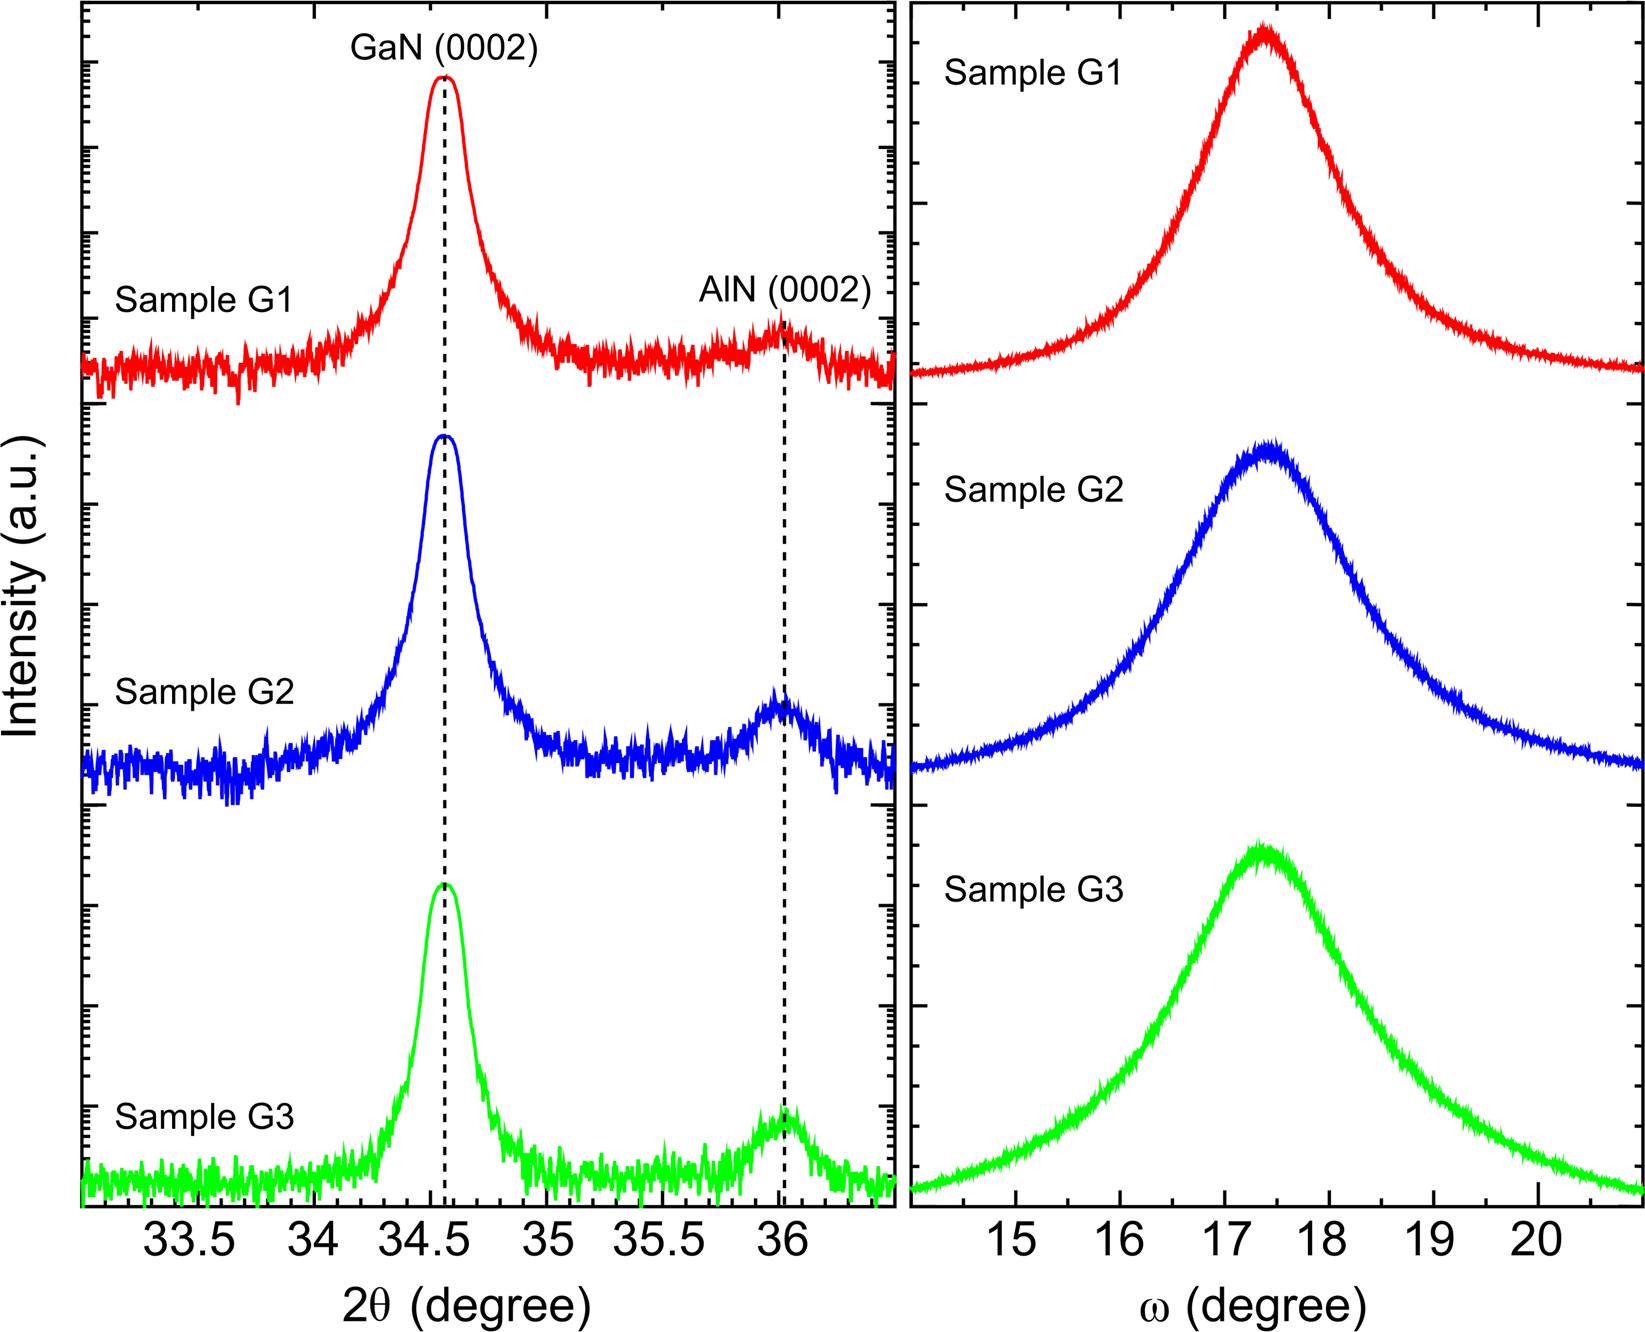
\includegraphics[width=\textwidth]{figures/paper-iv/fig-6.png}
    \caption[HRXRD measurements of the nanocolumns]{HRXRD measurements of the nanocolumns. (\textbf{a}) 2\straighttheta-\textomega \ scanning curve and (\textbf{b}) \textomega \ scanning curve of samples G1, G2 and G3 (adapted with permission from ref. \citenum{liudimulyo2020853} \copyright \ Liudi Mulyo \textit{et al}, 2020.}
    \label{fig:figures/paper-iv/fig-6}
\end{figure}

\section{Section 1 in chapter 6}
\lipsum[2-4]

\subsection{Subsection 6.1 of section 1 in chapter 6}
\lipsum[5-7]

\subsection{Subsection 6.2 of section 1 in chapter 6}
\lipsum[8-11]

\clearpage\phantomsection % to fix wrong hyperref to this section
\section[Long section title displayed in the table of content]{Short section title in the chapter}
\sectionmark{Even shorter title on the header}
\lipsum[11-18]
See \ref{tab:ch6}

\begin{table}[H]
\centering
\caption[Al-content of each axial nanocolumn segment for the vertical GaN/AlGaN nanocolumn ensemble obtained from fitting the simulation model to the HRXRD 2\straighttheta-\textomega \ scan data]{Al-content of each axial nanocolumn segment for the vertical GaN/AlGaN nanocolumn ensemble (top to bottom) obtained from fitting the simulation model to the HRXRD 2\straighttheta-\textomega \ scan data}
\label{tab:ch6}
{\fontsize{7}{6}\selectfont
{\renewcommand{\arraystretch}{2}
\begin{tabular}{cccc}
\textbf{Segment} & \textbf{Thickness (nm)} & \textbf{Al bottom (\%)} & \textbf{Al top (\%)} \\
\midrule
\begin{tabular}[c]{@{}c@{}}\textit{p-}GaN\end{tabular} & 1 & 2 & 3 \\
\rowcolor{Gray}\begin{tabular}[c]{@{}c@{}}\textit{p-}AlGaN (linear grading)\end{tabular} & 4 & 5 & 6 \\
\begin{tabular}[c]{@{}c@{}}\textit{i-}GaN quantum disk\end{tabular} & 7 & 8 & 9 \\
\rowcolor{Gray}\begin{tabular}[c]{@{}c@{}}\textit{n-}AlGaN (linear grading)\end{tabular} & 10 & 11 & 12 \\
\begin{tabular}[c]{@{}c@{}}\textit{n-}GaN\end{tabular} & 13 & 14 & 15 \\
\rowcolor{Gray}\begin{tabular}[c]{@{}c@{}}\textit{n-}AlN buffer layer\end{tabular} & 16 & 17 & 18 \\
\end{tabular}
}
}
\end{table}

\subsection{Subsection 6.2 of section 2 in chapter 6}
\label{subsec:labelsubsec6-2}
\lipsum[13-14]
See \hyperref[appendix:C]{Appendix C} for the \ref{fig:figures/paper-iv/fig-7} and \ref{fig:figures/paper-iv/fig-8}.

%=======================================================================
%%% References 

% \clearpage
\phantomsection
\specialsection % put an indent, see preamble
\headerspecialsection

{\hypersetup{urlcolor=ntnu,linkcolor=sophia} % set clickable URL title color to black, not ntnu like in the main document

\bibliographystyle{unsrtnat-mod}  % NATBIB ref style
\bibliography{references}
}

\cleardoublepage\phantomsection % to fix wrong hyperref to \part{Epilogue}
\part{Epilogue}

\chapter[Conclusion]{Conclusion}
\markboth{Chap. 7\ \ \enspace Conclusion}{Chap 7. Conclusion}

\regularsection
\headerregularsection

\begin{sloppypar} % to suppress overfull box

Lorem \index{Lorem} ipsum dolor sit amet, consectetuer adipiscing elit \cite{LIUDIMULYO201767}. Ut purus \index{purus} elit,vestibulum ut, placerat ac, adipiscing vitae, felis \citenum{LIUDIMULYO201767}. Curabitur dictum \index{dictum} gravidamauris. Nam arcu libero, nonummy eget, consectetuer id, vulputate a, magna. Donec vehicula augue eu neque \cite{liudimulyo_2018}. Pellentesque habitant morbi tristique senectuset netus et malesuada fames ac turpis egestas \index{egestas}\citenum{liudimulyo_2018}. Mauris ut leo. Cras viverra metusrhoncus sem \cite{2019liudimulyo}. Nulla et lectus vestibulum urna fringilla ultrices. Phasellus eutellus sit amet tortor gravida placerat \citenum{2019liudimulyo}. Integer sapien est, iaculis in, pretium quis,viverra ac, nunc. Praesent eget sem vel leo ultrices bibendum \cite{liudimulyo2020853}. Aenean faucibus. Morbi dolor nulla, malesuada eu, pulvinar at (\ref{fig:figures/paper-iv/fig-1}), mollis ac, nulla. Curabitur auctorsemper nulla \citenum{liudimulyo2020853}. Donec varius orci eget risus. Duis nibh mi, congue eu, accumsaneleifend, sagittis quis, diam. Duis eget orci sit amet orci dignissim rutrum \cite{LIUDIMULYO201767,liudimulyo_2018,2019liudimulyo,liudimulyo2020853,liudimulyo_unpublished1,liudimulyo_unpublished2}. For \Autoref{ch:labelchapter4} and \Autoref{ch:labelchapter5}, as well as \Autoref{ch:labelchapter6}

\end{sloppypar}

\section{Section 1 in chapter 7}
\lipsum[2-4]

\subsection{Subsection 7.1 of section 1 in chapter 7}
\lipsum[5-7]

\subsection{Subsection 7.2 of section 1 in chapter 7}
\lipsum[8-11]

\clearpage\phantomsection % to fix wrong hyperref to this section
\section[Long section title displayed in the table of content]{Short section title in the chapter}
\sectionmark{Even shorter title on the header}
\lipsum[11-19]

\subsection{Subsection 7.2 of section 2 in chapter 7}
\lipsum[13-14]

%=======================================================================
%%% References 

% \clearpage
\phantomsection
\specialsection % put an indent, see preamble
\headerspecialsection

{\hypersetup{urlcolor=ntnu,linkcolor=sophia} % set clickable URL title color to black, not ntnu like in the main document

\bibliographystyle{unsrtnat-mod}  % NATBIB ref style
\bibliography{references}
}

%=======================================================================

\vspace{2.81ex}

\begin{center}
    {\color{sophia} \Huge
    \adforn{21}
    }
\end{center}

\clearpage\null\thispagestyle{empty}

%=======================================================================

%%% Back matter
\backmatter

%%% Appendix A

\chapter[Appendix A \hspace{0.0025em} Supplementary information for chapter 4]{\textsc{Appendix A} \vspace{8pt} \\ Supporting information for chapter 4}

\label{appendix:A}

\setcounter{page}{1}
\renewcommand{\thepage}{A-\arabic{page}}

\setcounter{chapter}{0}
\renewcommand{\thechapter}{\Alph{chapter}}
\renewcommand{\theHchapter}{A\thechapter}

\setcounter{section}{0}
\renewcommand{\thesection}{A.\arabic{section}}

\setcounter{figure}{0}
\renewcommand{\thefigure}{A.\arabic{figure}}

\setcounter{table}{0}
\renewcommand{\thetable}{A.\arabic{table}}

% \updatemylofappendixA % uncomment this if this appendix has figure -> ToC will be updated
\updatemylotappendixA

\markboth{Appendix A \hspace{0.0025em} Supplementary information for chapter 4}
{Appendix A \hspace{0.0025em} Supplementary information for chapter 4}

\regularsection
\headerspecialsectionappendix

% ============================================================================================================

\section{Detailed growth information}

\begin{sloppypar} % to suppress overfull box

Lorem \index{Lorem} ipsum dolor sit amet, consectetuer adipiscing elit \cite{LIUDIMULYO201767}. Ut purus \index{purus} elit,vestibulum ut, placerat ac, adipiscing vitae, felis \citenum{LIUDIMULYO201767}. Curabitur dictum \index{dictum} gravidamauris. Nam arcu libero, nonummy eget, consectetuer id, vulputate a, magna. Donec vehicula augue eu neque \cite{liudimulyo_2018}. Pellentesque habitant morbi tristique senectuset netus et malesuada fames ac turpis egestas \index{egestas}\citenum{liudimulyo_2018}. Mauris ut leo. Cras viverra metusrhoncus sem \cite{2019liudimulyo}. Nulla et lectus vestibulum urna fringilla ultrices. Phasellus eutellus sit amet tortor gravida placerat \citenum{2019liudimulyo}. Integer sapien est, iaculis in, pretium quis,viverra ac, nunc. Praesent eget sem vel leo ultrices bibendum \cite{liudimulyo2020853}. Aenean faucibus. Morbi dolor nulla, malesuada eu, pulvinar at (\ref{fig:figures/paper-iv/fig-4}), mollis ac, nulla. Curabitur auctorsemper nulla \citenum{liudimulyo2020853}. Donec varius orci eget risus. Duis nibh mi, congue eu, accumsaneleifend, sagittis quis, diam. Duis eget orci sit amet orci dignissim rutrum \cite{LIUDIMULYO201767,liudimulyo_2018,2019liudimulyo,liudimulyo2020853,liudimulyo_unpublished1,liudimulyo_unpublished2}.

\end{sloppypar}

\begin{table}[!h]
\centering
\caption{Detailed growth conditions of nanocolumns} % use this to compensate "from tcbcaption to break the long sentence" in PREAMBLE instead if the "default" one
\label{tab:appendixA}
\rotatebox{90}{
\begin{minipage}{17cm}
\centering
{\renewcommand{\arraystretch}{1.5}
\begin{tabular}{cccccccc}
\toprule
\multirow{3}{*}{\textbf{\begin{tabular}[c]{@{}c@{}} Nanocolumn\\ segment/layer \\\end{tabular}}} & \multirow{2}{*}{\textbf{\begin{tabular}[c]{@{}c@{}} Growth temperature, \\ pyrometer reading \\ ($^\circ$C)\end{tabular}}} & 
\multicolumn{3}{c}{\textbf{\begin{tabular}[c]{@{}c@{}} Beam equivalent pressure (Pa)\end{tabular}}} & \multirow{2}{*}{\textbf{\begin{tabular}[c]{@{}c@{}}Si cell\\ temperature\\ ($^\circ$C)\end{tabular}}} & \multirow{2}{*}{\textbf{\begin{tabular}[c]{@{}c@{}}N\textsubscript{2} flow rate/ \\ plasma emission\\  (sccm/mV)\end{tabular}}} & 
\multirow{3}{*}{\textbf{\begin{tabular}[c]{@{}c@{}} Growth time\\ (sec)\end{tabular}}} \\
\cmidrule(l){3-5} \cmidrule(l){3-5} \cmidrule(l){3-5} % repeated three times to increase the line thickness
 &  & \multirow{2}{*}{\textbf{\begin{tabular}[c]{@{}c@{}}Al\end{tabular}}} & \multirow{2}{*}{\textbf{\begin{tabular}[c]{@{}c@{}}Ga\end{tabular}}} & \multirow{2}{*}{\textbf{\begin{tabular}[c]{@{}c@{}}Mg\end{tabular}}} &  &  &  \\
\multicolumn{1}{l}{} & \multicolumn{1}{l}{} & \multicolumn{1}{l}{} & \multicolumn{1}{l}{} & \multicolumn{1}{l}{} & \multicolumn{1}{l}{} & \multicolumn{1}{l}{} & \multicolumn{1}{l}{} \\
\midrule
\begin{tabular}[c]{@{}c@{}} 
Al seeding\\ with Si\end{tabular} & 1 & 2.0 $\times$ 10\textsuperscript{-3} & - & - & 4 & - & 5 \\

\cellcolor{Gray} & \cellcolor{Gray} & \cellcolor{Gray} & \cellcolor{Gray} & \cellcolor{Gray} & \cellcolor{Gray} & \cellcolor{Gray} & \cellcolor{Gray} \\
\multirow{-2}{*}{\cellcolor{Gray} Nitridation} & \multirow{-2}{*}{\cellcolor{Gray} 6} & \multirow{-2}{*}{\cellcolor{Gray} -} & \multirow{-2}{*}{\cellcolor{Gray} -} & \multirow{-2}{*}{\cellcolor{Gray} -} & \multirow{-2}{*}{\cellcolor{Gray} -} & \multirow{-2}{*}{\cellcolor{Gray} 7.00/8.9} & \multirow{-2}{*}{\cellcolor{Gray} 1} \\

\cellcolor{White} & \cellcolor{White} & \cellcolor{White} & \cellcolor{White} & \cellcolor{White} & \cellcolor{White} & \cellcolor{White} & \cellcolor{White} \\
\multirow{-2}{*}{\cellcolor{White} n-AlN} & \multirow{-2}{*}{\cellcolor{White} 2} & \multirow{-2}{*}{\cellcolor{White} 3.0 $\times$ 10\textsuperscript{-4}} & \multirow{-2}{*}{\cellcolor{White} -} & \multirow{-2}{*}{\cellcolor{White} -} & \multirow{-2}{*}{\cellcolor{White} 5} & \multirow{-2}{*}{\cellcolor{White} 6.00/7.89} & \multirow{-2}{*}{\cellcolor{White} 1} \\

\cellcolor{Gray} & \cellcolor{Gray} & \cellcolor{Gray} & \cellcolor{Gray} & \cellcolor{Gray} & \cellcolor{Gray} & \cellcolor{Gray} & \cellcolor{Gray} \\
\multirow{-2}{*}{\cellcolor{Gray} n-GaN} & \multirow{-2}{*}{\cellcolor{Gray} 2} & \multirow{-2}{*}{\cellcolor{Gray} -} & \multirow{-2}{*}{\cellcolor{Gray} 3.4 $\times$ 10\textsuperscript{-5}} & \multirow{-2}{*}{\cellcolor{Gray} -} & \multirow{-2}{*}{\cellcolor{Gray} 6} & \multirow{-2}{*}{\cellcolor{Gray} 7.89/1.23} & \multirow{-2}{*}{\cellcolor{Gray} 4} \\

\cellcolor{White} & \cellcolor{White} & \cellcolor{White} & \cellcolor{White} & \cellcolor{White} & \cellcolor{White} & \cellcolor{White} & \cellcolor{White} \\
\multirow{-2}{*}{\cellcolor{White} n-Al\textsubscript{0.56}Ga\textsubscript{0.78}N} & \multirow{-2}{*}{\cellcolor{White} 9} & \multirow{-2}{*}{\cellcolor{White} 1.2 $\times$ 10\textsuperscript{-3}} & \multirow{-2}{*}{\cellcolor{White} 4.0 $\times$ 10\textsuperscript{-5}} & \multirow{-2}{*}{\cellcolor{White} -} & \multirow{-2}{*}{\cellcolor{White} 6} & \multirow{-2}{*}{\cellcolor{White} 7.00/8.9} & \multirow{-2}{*}{\cellcolor{White} 1} \\

\cellcolor{Gray} & \cellcolor{Gray} & \cellcolor{Gray} & \cellcolor{Gray} & \cellcolor{Gray} & \cellcolor{Gray} & \cellcolor{Gray} & \cellcolor{Gray} \\
\multirow{-2}{*}{\cellcolor{Gray} i-GaN} & \multirow{-2}{*}{\cellcolor{Gray} 2} & \multirow{-2}{*}{\cellcolor{Gray} -} & \multirow{-2}{*}{\cellcolor{Gray} 3.1 $\times$ 10\textsuperscript{-2}} & \multirow{-2}{*}{\cellcolor{Gray} -} & \multirow{-2}{*}{\cellcolor{Gray} -} & \multirow{-2}{*}{\cellcolor{Gray} 3.45/6.78} & \multirow{-2}{*}{\cellcolor{Gray} 9} \\

\cellcolor{White} & \cellcolor{White} & \cellcolor{White} & \cellcolor{White} & \cellcolor{White} & \cellcolor{White} & \cellcolor{White} & \cellcolor{White} \\
\multirow{-2}{*}{\cellcolor{White} p-Al\textsubscript{1.23}Ga\textsubscript{4.56}N} & \multirow{-2}{*}{\cellcolor{White} 7} & \multirow{-2}{*}{\cellcolor{White} 8.9 $\times$ 10\textsuperscript{-1}} & \multirow{-2}{*}{\cellcolor{White} 2.0 $\times$ 10\textsuperscript{-3}} & \multirow{-2}{*}{\cellcolor{White} 4.0 $\times$ 10\textsuperscript{-5}} & \multirow{-2}{*}{\cellcolor{White} -} & \multirow{-2}{*}{\cellcolor{White} 6.00/7.89} & \multirow{-2}{*}{\cellcolor{White} 1} \\

\cellcolor{Gray} & \cellcolor{Gray} & \cellcolor{Gray} & \cellcolor{Gray} & \cellcolor{Gray} & \cellcolor{Gray} & \cellcolor{Gray} & \cellcolor{Gray} \\
\multirow{-2}{*}{\cellcolor{Gray} p-GaN} & \multirow{-2}{*}{\cellcolor{Gray} 2} & \multirow{-2}{*}{\cellcolor{Gray} -} & \multirow{-2}{*}{\cellcolor{Gray} 3.0 $\times$ 10\textsuperscript{-4}} & \multirow{-2}{*}{\cellcolor{Gray} 5.0 $\times$ 10\textsuperscript{-6}} & \multirow{-2}{*}{\cellcolor{Gray} -} & \multirow{-2}{*}{\cellcolor{Gray} 7.00/8.9} & \multirow{-2}{*}{\cellcolor{Gray} 1} \\
\bottomrule
\end{tabular}
}
\end{minipage}
}
\end{table}

%=======================================================================
%%% References 

\clearpage
\phantomsection
\specialsection
\headerspecialsection

{\hypersetup{urlcolor=ntnu,linkcolor=sophia} % set clickable URL title color to black, not blue like in the main document

\bibliographystyle{unsrtnat-mod} % NATBIB ref style
\bibliography{references}
}

%=======================================================================
%%% Appendix B

\chapter[Appendix B \hspace{0.0025em} Supplementary information for chapter 5]{\textsc{Appendix B} \vspace{8pt} \\ Supporting information for chapter 5}

\label{appendix:B}

\setcounter{chapter}{0}
\renewcommand{\thechapter}{\Alph{chapter}}
\renewcommand{\theHchapter}{B\thechapter}

\setcounter{section}{0}
\renewcommand{\thesection}{B.\arabic{section}}

\setcounter{figure}{0}
\renewcommand{\thefigure}{B.\arabic{figure}}

\setcounter{table}{0}
\renewcommand{\thetable}{B.\arabic{table}}

% \updatemylofappendixB % uncomment this if this appendix has figure -> ToC will be updated
\updatemylotappendixB

\markboth{Appendix B \hspace{0.0025em} Supplementary information for chapter 5}
{Appendix B \hspace{0.0025em} Supplementary information for chapter 5}

\regularsection
\headerspecialsectionappendix

% ============================================================================================================

\section{Additional micro-Raman spectroscopy measurements}

\begin{sloppypar} % to suppress overfull box

Lorem \index{Lorem} ipsum dolor sit amet, consectetuer adipiscing elit \cite{LIUDIMULYO201767}. Ut purus \index{purus} elit,vestibulum ut, placerat ac, adipiscing vitae, felis \citenum{LIUDIMULYO201767}. Curabitur dictum \index{dictum} gravidamauris. Nam arcu libero, nonummy eget, consectetuer id, vulputate a, magna. Donec vehicula augue eu neque \cite{liudimulyo_2018}. Pellentesque habitant morbi tristique senectuset netus et malesuada fames ac turpis egestas \index{egestas}\citenum{liudimulyo_2018}. Mauris ut leo. Cras viverra metusrhoncus sem \cite{2019liudimulyo}. Nulla et lectus vestibulum urna fringilla ultrices. Phasellus eutellus sit amet tortor gravida placerat \citenum{2019liudimulyo}. Integer sapien est, iaculis in, pretium quis,viverra ac, nunc. Praesent eget sem vel leo ultrices bibendum \cite{liudimulyo2020853}. Aenean faucibus. Morbi dolor nulla, malesuada eu, pulvinar at (\ref{fig:figures/paper-iv/fig-5}), mollis ac, nulla. Curabitur auctorsemper nulla \citenum{liudimulyo2020853}. Donec varius orci eget risus. Duis nibh mi, congue eu, accumsaneleifend, sagittis quis, diam. Duis eget orci sit amet orci dignissim rutrum \cite{LIUDIMULYO201767,liudimulyo_2018,2019liudimulyo,liudimulyo2020853,liudimulyo_unpublished1,liudimulyo_unpublished2}.

\end{sloppypar}

\begin{table}[!h]
\centering
\caption[Summary of micro-Raman spectroscopy measurements for the as-grown nanocolumn sample]{Summary of micro-Raman spectroscopy measurements for the as-grown nanocolumn sample carried out in different areas (of the same sample) from what is presented in \ref{fig:figures/paper-iv/fig-8}. The table shows the median values of the D peak, G peak, and 2D peak, for the entire mapping (123 measurements), from the green patches (45 measurements), and from the purple areas (67 measurements).}
\label{tab:appendixB}
{\fontsize{7}{6}\selectfont
{\renewcommand{\arraystretch}{2}
\begin{tabular}{cccccc}
\toprule
\multirow{2}{*}{\textbf{\begin{tabular}[c]{@{}c@{}}Median\\ value\end{tabular}}} & 
\multirow{2}{*}{\textbf{\begin{tabular}[c]{@{}c@{}}Area (number of\\ measurements)\end{tabular}}} & 
\multirow{2}{*}{\textbf{\begin{tabular}[c]{@{}c@{}}Position\\ {[} cm\textsuperscript{-1} {]}\end{tabular}}} & 
\multirow{2}{*}{\textbf{\begin{tabular}[c]{@{}c@{}}Intensity\\ {[} cps {]}\end{tabular}}} & 
\multirow{2}{*}{\textbf{\begin{tabular}[c]{@{}c@{}}FWHM\\ {[} cm\textsuperscript{-1} {]}\end{tabular}}} & 
\multirow{2}{*}{\textbf{\begin{tabular}[c]{@{}c@{}}Intensity ratio\\ to G peak\end{tabular}}}
\\
\\
\midrule

\multirow{3}{*}{\textbf{D peak}} & Green patches (45) & 1 & 2 & 3 & 4 \\
 & Full map (123) & 5 & 6 & 7 & 8 \\
 & Purple areas (67) & 9 & 1 & 2 & 3 \\

\cellcolor{Gray} & {\cellcolor{Gray}Green patches (45)} & {\cellcolor{Gray}4} & {\cellcolor{Gray}5} & {\cellcolor{Gray}-} & {\cellcolor{Gray}-} \\
\cellcolor{Gray} & {\cellcolor{Gray}Full map (123)} & {\cellcolor{Gray}6} & {\cellcolor{Gray}7} & {\cellcolor{Gray}-} & {\cellcolor{Gray}-} \\
\multirow{-3}{*}{\cellcolor{Gray}\textbf{G peak (*)}} & {\cellcolor{Gray}Purple areas (67)} & {\cellcolor{Gray}8} & {\cellcolor{Gray}9} & {\cellcolor{Gray}-} & {\cellcolor{Gray}-} \\

\multirow{3}{*}{\textbf{2D peak}} & Green patches (45) & 1 & 2 & 3 & 4 \\
 & Full map (123) & 5 & 6 & 7 & 8 \\
 & Purple areas (67) & 9 & 1 & 2 & 3 \\

\rowcolor{Gray}\textbf{D' peak (**)} & Green patches (45) & 4 & 5 & - & 6 \\ 

\bottomrule

\end{tabular}
}
}
\end{table}

%=======================================================================
%%% References 

\clearpage
\phantomsection
\specialsection
\headerspecialsection

{\hypersetup{urlcolor=ntnu,linkcolor=sophia} % set clickable URL title color to black, not blue like in the main document

\bibliographystyle{unsrtnat-mod} % NATBIB ref style
\bibliography{references}
}

%=======================================================================
%%% Appendix C

\chapter[Appendix C \hspace{0.0025em} Supplementary information for chapter 6]{\textsc{Appendix C} \vspace{8pt} \\ Supplementary information for chapter 6}

\label{appendix:C}

\setcounter{chapter}{0}
\renewcommand{\thechapter}{\Alph{chapter}}
\renewcommand{\theHchapter}{C\thechapter}

\setcounter{section}{0}
\renewcommand{\thesection}{C.\arabic{section}}

\setcounter{figure}{0}
\renewcommand{\thefigure}{C.\arabic{figure}}

\setcounter{table}{0}
\renewcommand{\thetable}{C.\arabic{table}}

\updatemylofappendixC
% \updatemylotappendixC % uncomment this if this appendix has table -> ToC will be updated

\markboth{Appendix C \hspace{0.0025em} Supplementary information for chapter 6}%
{Appendix C \hspace{0.0025em} Supplementary information for chapter 6}

\regularsection
\headerspecialsectionappendix

% ============================================================================================================

\section[micro-PL spectra]{micro-photoluminescence spectra of HVPE-GaN and nanocolumn samples}

This is an additional characterization from \Autoref{subsec:labelsubsec6-2}.

\begin{figure}[H]
    \centering
    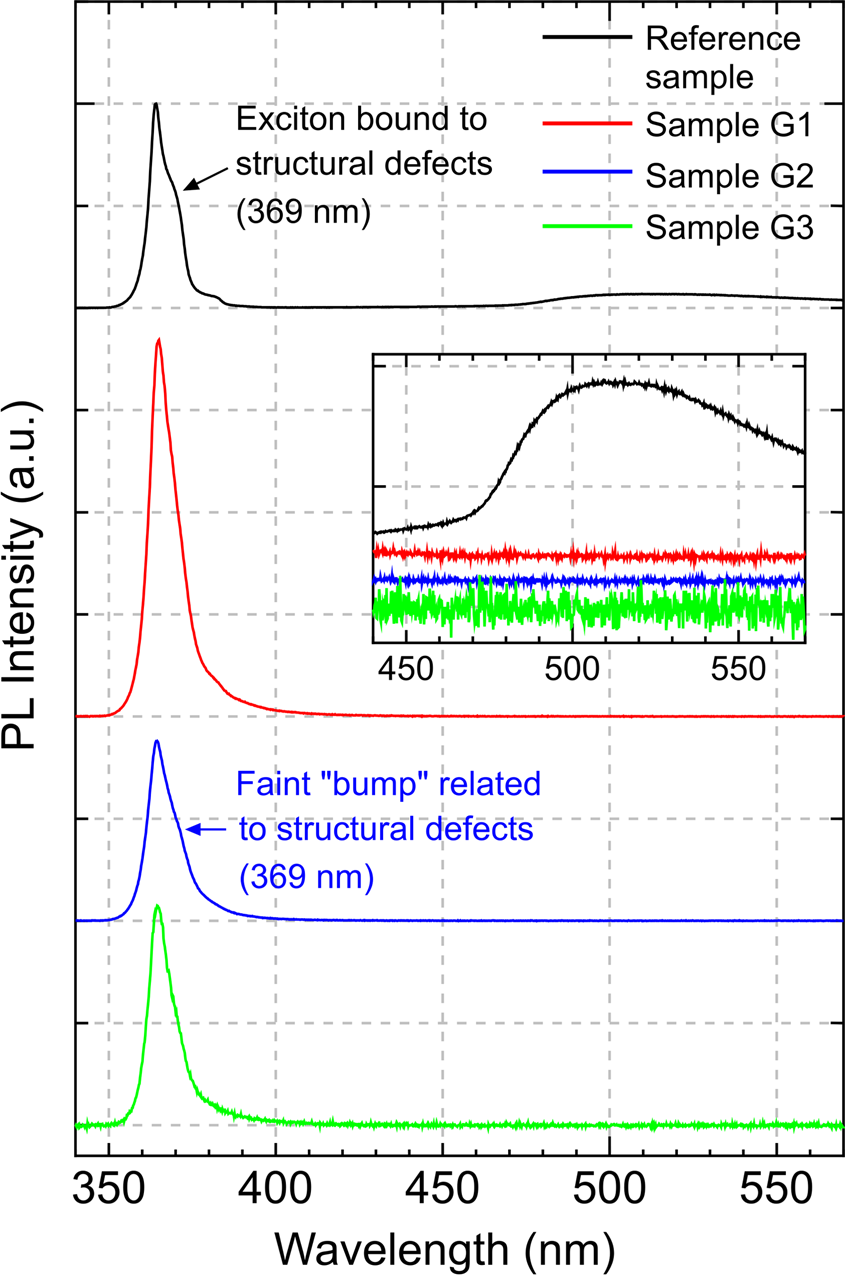
\includegraphics[width=0.6\textwidth]{figures/paper-iv/fig-7.png}
    \caption[RT micro-photoluminescence spectra of reference sample\newline (HVPE-freestanding GaN), samples G1, G2 and G3]{RT micro-photoluminescence spectra of reference sample (HVPE-freestanding GaN), samples G1, G2 and G3. Inset shows the magnified spectra in the wavelength range from 440 to 570 nm, highlighting the presence of broad green and yellow emission band in the reference sample (adapted with permission from ref. \citenum{liudimulyo2020853} \copyright \ Liudi Mulyo \textit{et al}, 2020.}
    \label{fig:figures/paper-iv/fig-7}
\end{figure}

\newpage

\section[micro-Raman spectra]{micro-Raman spectra of pristine graphene and nanocolumn samples after growth}

This is an extra measurement from \autoref{subsec:labelsubsec6-2}

\begin{figure}[H]
    \centering
    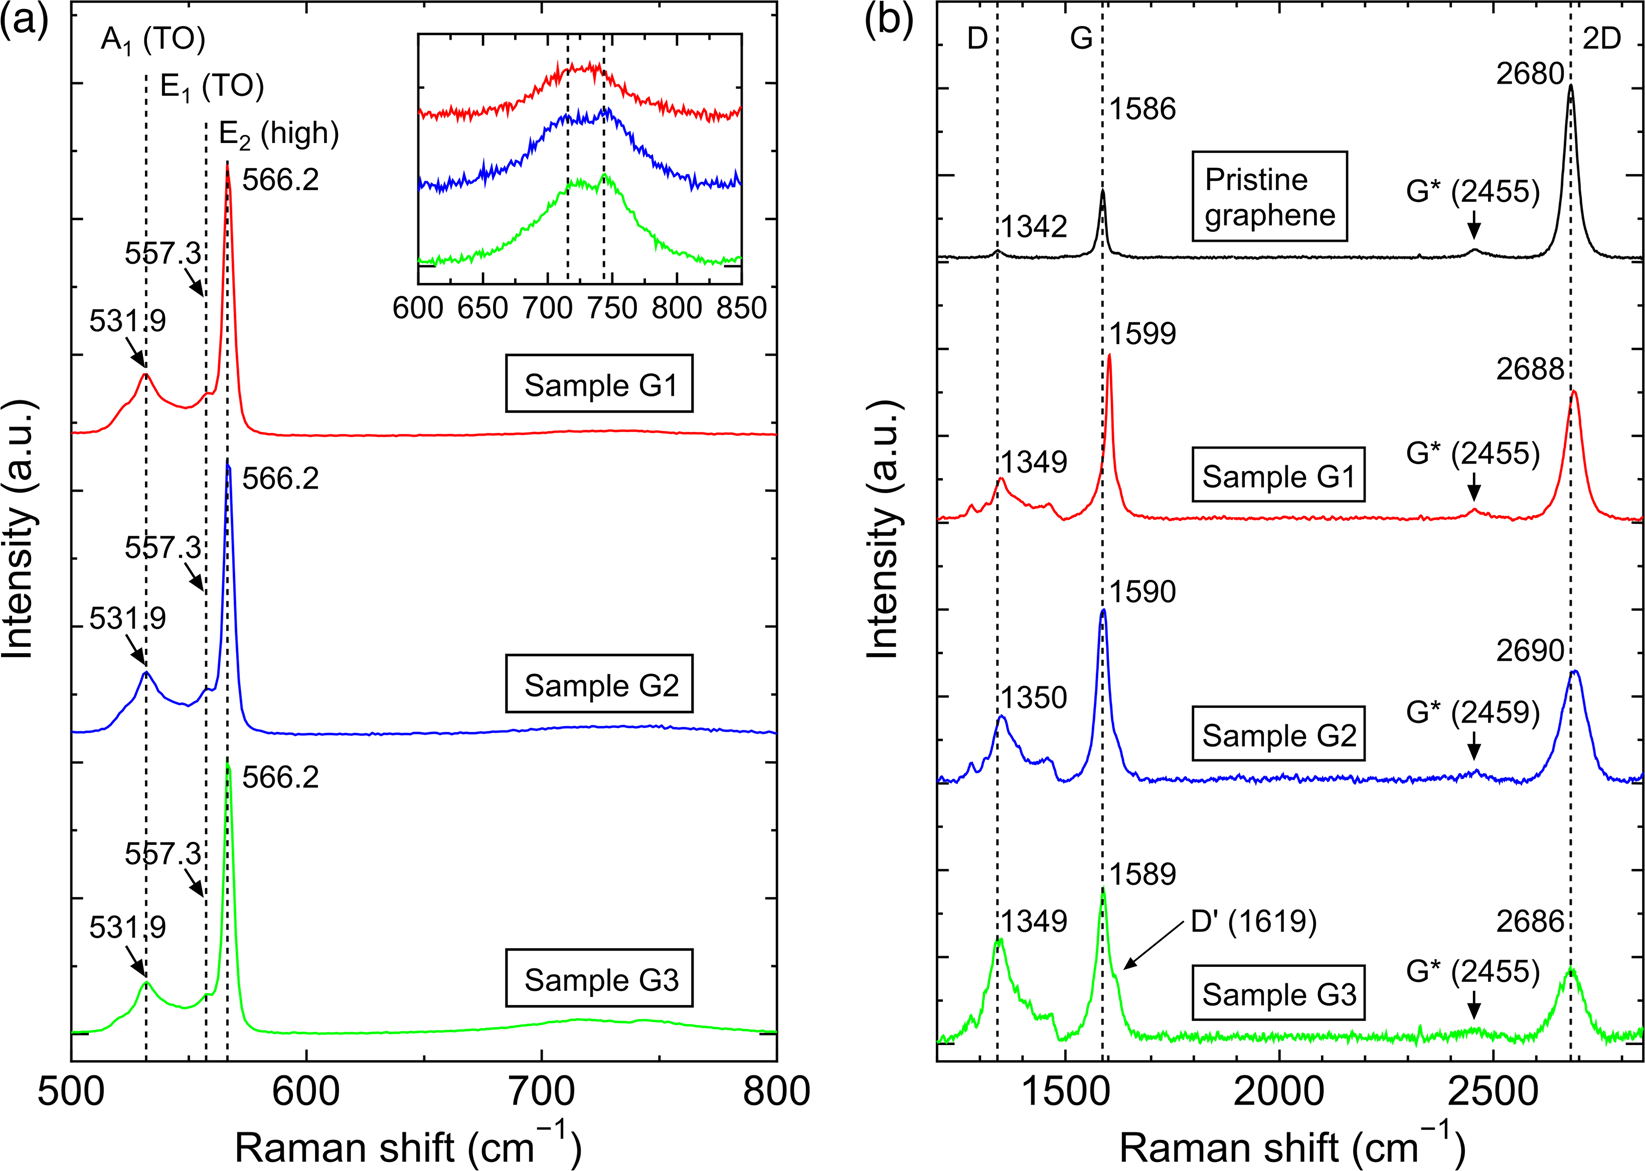
\includegraphics[width=\textwidth]{figures/paper-iv/fig-8.png}
    \caption[Micro-Raman spectroscopy of the nanocolumn samples,\newline including the graphene for each respective sample]{Micro-Raman spectroscopy of the nanocolumn samples, including the graphene for each respective sample. Raman spectra of (\textbf{a}) samples G1, G2 and G3 between 500 and 800 cm\textsuperscript{-1}, with the peak frequencies of the A\textsubscript{1} (TO), E\textsubscript{1} (TO) and E\textsubscript{2} (high) modes indicated by vertical dashed lines (inset: magnification from 600 to 850 cm\textsuperscript{-1}, with the identified peak frequencies at 715 and 743 cm\textsuperscript{-1} of the possible SO and LPP modes, respectively \cite{2016robins,2009jeganathan}, indicated by vertical dashed lines), and (\textbf{b}) pristine graphene, samples G1, G2 and G3 between 1100 and 3200 cm\textsuperscript{-1}. The dashed lines indicate D, G and 2D peak positions of pristine graphene (adapted with permission from ref. \citenum{liudimulyo2020853} \copyright \ Liudi Mulyo \textit{et al}, 2020.}
    \label{fig:figures/paper-iv/fig-8}
\end{figure}

%=======================================================================
%%% References 

\clearpage
\phantomsection
\specialsection
\headerspecialsection

{\hypersetup{urlcolor=ntnu,linkcolor=sophia} % set clickable URL title color to black, not blue like in the main document

\bibliographystyle{unsrtnat-mod} % NATBIB ref style
\bibliography{references}
}

%=======================================================================
%%% Curriculum vitae

\chapter[Curriculum vitae]{\textsc{Curriculum vitae} \vspace{8pt} \\ Author}

\setcounter{page}{1}
\renewcommand{\thepage}{L-\arabic{page}}

\markboth{Curriculum vitae}%
{Curriculum vitae}

\regularsection
\headerregularsection

% ============================================================================================================

{\color{sophia} \small \bfseries \fontfamily{bch} \selectfont \scshape Personal information} \vspace{4mm}

\noindent Family name, given name \hspace{3mm} : \hspace{2.4mm} Author \\
Nationaliy \hspace{25mm} : \hspace{2.4mm} Citizenship 
\\
Place, date of birth \hspace{13mm} : \hspace{2.4mm} City (Country), Month date\textsuperscript{st/nd/rd/th}, yyyy
\\
Current address \hspace{16.7mm} : \hspace{2.4mm} Address, Postal code City, NO 

% =====================================================

\begin{adjustwidth}{0cm}{1cm}
{\vspace{4mm} \color{sophia} \small \bfseries \fontfamily{bch} \selectfont \scshape Educational background and research experience} \vspace{4mm}
\end{adjustwidth}

\noindent \textbf{Doctor of Philosophy (Ph.D.)} in Electronic Systems\\ Norwegian University of Science and Technology (NTNU), Trondheim, NO\\ month yyyy - month 2021
    \vspace{-0.2cm}
    \begin{itemize}[itemsep=0.7pt, parsep=0.7pt, leftmargin=7mm, label=\adforn{43}] % or alternatively (not rotated), \footnotesize\ding{} 121, 122, 117, 118, 114, 212
        \item Thesis title: The title of PhD thesis
        \item Advisors: Professor Supervisor and Professor Co-supervisor
        \item Additional information, like collaborative researcher at another Laboratory (name of the Professor) at University X, City, Country for total of xx months
    \end{itemize}
    \vspace{0.5mm}
    
\noindent \textbf{Master of Science (M.Sc.)} in Condensed Matter Physics\\ Norwegian University of Science and Technology (NTNU), Trondheim, NO\\ month yyyy - month 2013
    \vspace{-0.2cm}
    \begin{itemize}[itemsep=0.7pt, parsep=0.7pt, leftmargin=7mm, label=\adforn{43}] % or alternatively (not rotated), \footnotesize\ding{} 121, 122, 117, 118, 114, 212
        \item Thesis title: The title of MSc thesis
        \item Advisors: Professor Supervisor and Professor Co-supervisor
    \end{itemize}
    \vspace{0.5mm}
    
\noindent \textbf{Bachelor of Engineering (B.Eng.)} in Engineering Physics\\ Norwegian University of Science and Technology (NTNU), Trondheim, NO\\ month yyyy - month 2010
    \vspace{-0.2cm}
    \begin{itemize}[itemsep=0.7pt, parsep=0.7pt, leftmargin=7mm, label=\adforn{43}] % or alternatively (not rotated), \footnotesize\ding{} 121, 122, 117, 118, 114, 212
        \item Thesis title: The title of BEng thesis
        \item Advisors: Professor Supervisor and Professor Co-supervisor
    \end{itemize}

% ============================================================================================================
\newpage

\begin{adjustwidth}{0cm}{1cm} % 
{\vspace{3mm} \color{sophia} \small \bfseries \fontfamily{bch} \selectfont \scshape Teaching experience} \vspace{3mm}
\end{adjustwidth}

\noindent Laboratory assistant for various courses, at \textbf{NTNU}: Nanoelectronics 2 (spring 2020 \& 2021), Semiconductor Physics with Lab (spring 2017-2020), Physical Methods for Nanostructuring and Characterization (autumn 2017 \& 2018), Chemical Methods for Synthesis and Characterization of Nanomaterial (autumn 2017 \& 2018).

% ============================================================================================================

\begin{adjustwidth}{0cm}{1cm} % 
{\vspace{3mm} \color{sophia} \small \bfseries \fontfamily{bch} \selectfont \scshape Awards} \vspace{1mm}
\end{adjustwidth}

\begin{itemize}[itemsep=0.7pt, parsep=0.7pt, leftmargin=7mm, label=\adforn{43}] % or alternatively (not rotated), \footnotesize\ding{} 121, 122, 117, 118, 114, 212
    \item Norges tekniske h{\o}gskoles fond, a travel grant for \href{http://ece.umich.edu/issled2017/}{ISSLED 2017} \hfill 2017
    \item NorFab travel grant for \href{https://mbe2016.sciencesconf.org/conference/mbe2016/pages/MBE2016_Final_program.pdf#page=42}{MBE 2016} and \href{http://www.csw2017.org}{CSW 2017} \hfill 2017-2018
    \item NorFab project support, for research visit in University X \hfill 2018-2019
    \item PhD scholarship, NTNU \hfill 2017-2021
\end{itemize}

% ============================================================================================================

\begin{adjustwidth}{0cm}{1cm} % 
{\vspace{2mm} \color{sophia} \small \bfseries \fontfamily{bch} \selectfont \scshape Skills} \vspace{3mm}
\end{adjustwidth}

\noindent Scientific (laboratory) competency
\vspace{-0.1cm}
\begin{itemize}[itemsep=0.7pt, parsep=0.7pt, leftmargin=7mm, label=\adforn{43}] % or alternatively (not rotated), \footnotesize\ding{} 121, 122, 117, 118, 114, 212
    \item Experienced with the growth of semiconductor using molecular beam epitaxy technique.
    \item Skilled for material characterization techniques using scanning electron microscopy, photoluminescence, and Raman spectroscopy.
    \item Familiar with device fabrication tools, including mask/maskless aligner, e-beam/sputter deposition, plasma-enhanced chemical vapor deposition, wet etching, and inductively-coupled plasma reactive ion etching. 
    \item Basic knowledge of e-beam lithography and X-ray diffraction.
\end{itemize}

\noindent Computer literacy
\vspace{-0.1cm}
\begin{itemize}[itemsep=0.7pt, parsep=0.7pt, leftmargin=7mm, label=\adforn{43}] % or alternatively (not rotated), \footnotesize\ding{} 121, 122, 117, 118, 114, 212
    \item Microsoft Windows, MacOS, and Debian-based Linux (competent)
    \item Microsoft Office, Inkscape, ImageJ, Ngraph, and \LaTeX \ (intermediate)
    \item SketchUp, Blender, Python, MatLab, \verb!C++!, HTML, and LabView (beginner)
    % (beginner)
\end{itemize}

\noindent Language fluency \\
    \begin{minipage}[t]{.5\linewidth}
        \vspace{-0.2cm}
        \begin{itemize}[itemsep=0.7pt, parsep=0.7pt, leftmargin=7mm, label=\adforn{43}] % or alternatively (not rotated), \footnotesize\ding{} 121, 122, 117, 118, 114, 212
            \item Indonesia (native)
            \item English (full professional)
        \end{itemize}
    \end{minipage}\hspace{0.1cm}
    \begin{minipage}[t]{.4\linewidth}
        \vspace{-0.2cm}
        \begin{itemize}[itemsep=0.5pt, parsep=0.7pt, leftmargin=7mm, label=\adforn{43}] % or alternatively (not rotated), \footnotesize\ding{} 121, 122, 117, 118, 114, 212
            \item Japanese (elementary)
            \item Norwegian (elementary)
        \end{itemize}
    \end{minipage}

% ============================================================================================================

\begin{adjustwidth}{0cm}{1cm} % 
{\vspace{4mm} \color{sophia} \small \bfseries \fontfamily{bch} \selectfont \scshape Contact information} \vspace{3mm}
\end{adjustwidth}

\noindent E-mail \hspace{30.8mm} : \hspace{2.4mm} \href{mailto:author@outlook.com}{author@outlook.com} \\
Homepage \hspace{24.9mm} : \hspace{2.4mm} \href{https://author.github.io}{https://author.github.io}
%%% Dissemination

\chapter{Dissemination of research}

\setcounter{figure}{0}
\renewcommand{\thefigure}{D.\arabic{figure}}

\updatemylofdissemination

\markboth{Dissemination of research}%
{Dissemination of research}

\regularsection
\headerregularsection

% to be used in the future
% https://tex.stackexchange.com/questions/297365/how-to-use-bibtex-for-putting-a-nice-publication-list-in-resume-with-document-cl
% https://gist.github.com/deparkes/3df4da19de3359dd0a1a59a59f9936cf
% https://tex.stackexchange.com/questions/97057/including-additional-bibliography-publication-list-in-thesis
% https://tex.stackexchange.com/questions/33008/what-is-the-most-convenient-way-to-create-annotated-bibliographies-e-g-in-a-li

% ============================================================================================================

{\color{sophia} \small \bfseries \fontfamily{bch} \selectfont \scshape Publications in peer reviewed journals}

\begin{enumerate}[wide=0em, leftmargin=*, labelsep=0.5em, widest=99, label={[\arabic*]}]

    \item \textbf{Author 1}, Author 2, Author 3, Author 4, Author 5, Author 6, and Author 7. \href{https://doi.org/10.1016/}{Title of the paper}. \textit{Journal of Crystal Growth} \textbf{480}, 67-73 (2017).
    
    \item \textbf{Author 1}, Author 2, Author 3, Author 4, Author 5, Author 6, and Author 7. \href{https://doi.org/10.1088/}{Title of paper 2}. \textit{Nanotechnology} \textbf{30} (1), 015604 (2018). \\
    \textit{This article was chosen as \textbf{cover image/featured article}, see \ref{fig:coverimage}.}
    
    \item Author 1\textcolor{red}{*}, \textbf{{Author 2}\textcolor{red}{*}}, Author 3, Author 4, Author 5, Author 6, Author 7, and Author 8. \href{https://doi.org/10.1021/}{Title of paper 3}. \textit{Nano Letters} \textbf{19} (3), 1649-1658 (2019). \\ \textcolor{red}{\textbf{*equal contributions}}
    
    \item \textbf{Author 1}, Author 2, Author 3, Author 4, Author 5, and Author 6. \href{https://doi.org/10.1038/}{Title of paper 4}. \textit{Scientific Reports} \textbf{10}, 853 (2020).
    
\end{enumerate}
 
{\color{sophia} \small \bfseries \fontfamily{bch} \selectfont \scshape \noindent Manuscript under review}

\begin{enumerate}[wide=0em, leftmargin=*, labelsep=0.5em, widest=99, label={[\arabic*]}]

    \item \textbf{Author 1}, Author 2\textcolor{red}{*}, Author 3\textcolor{red}{*}, Author 4, Author 5, Author 6, Author 7, Author 8, Author 9, and Author 10. \textcolor{ntnu}{Title of manuscript}. \\
    \textcolor{red}{*equal contributions}

\end{enumerate}

\begin{figure}
    \centering
    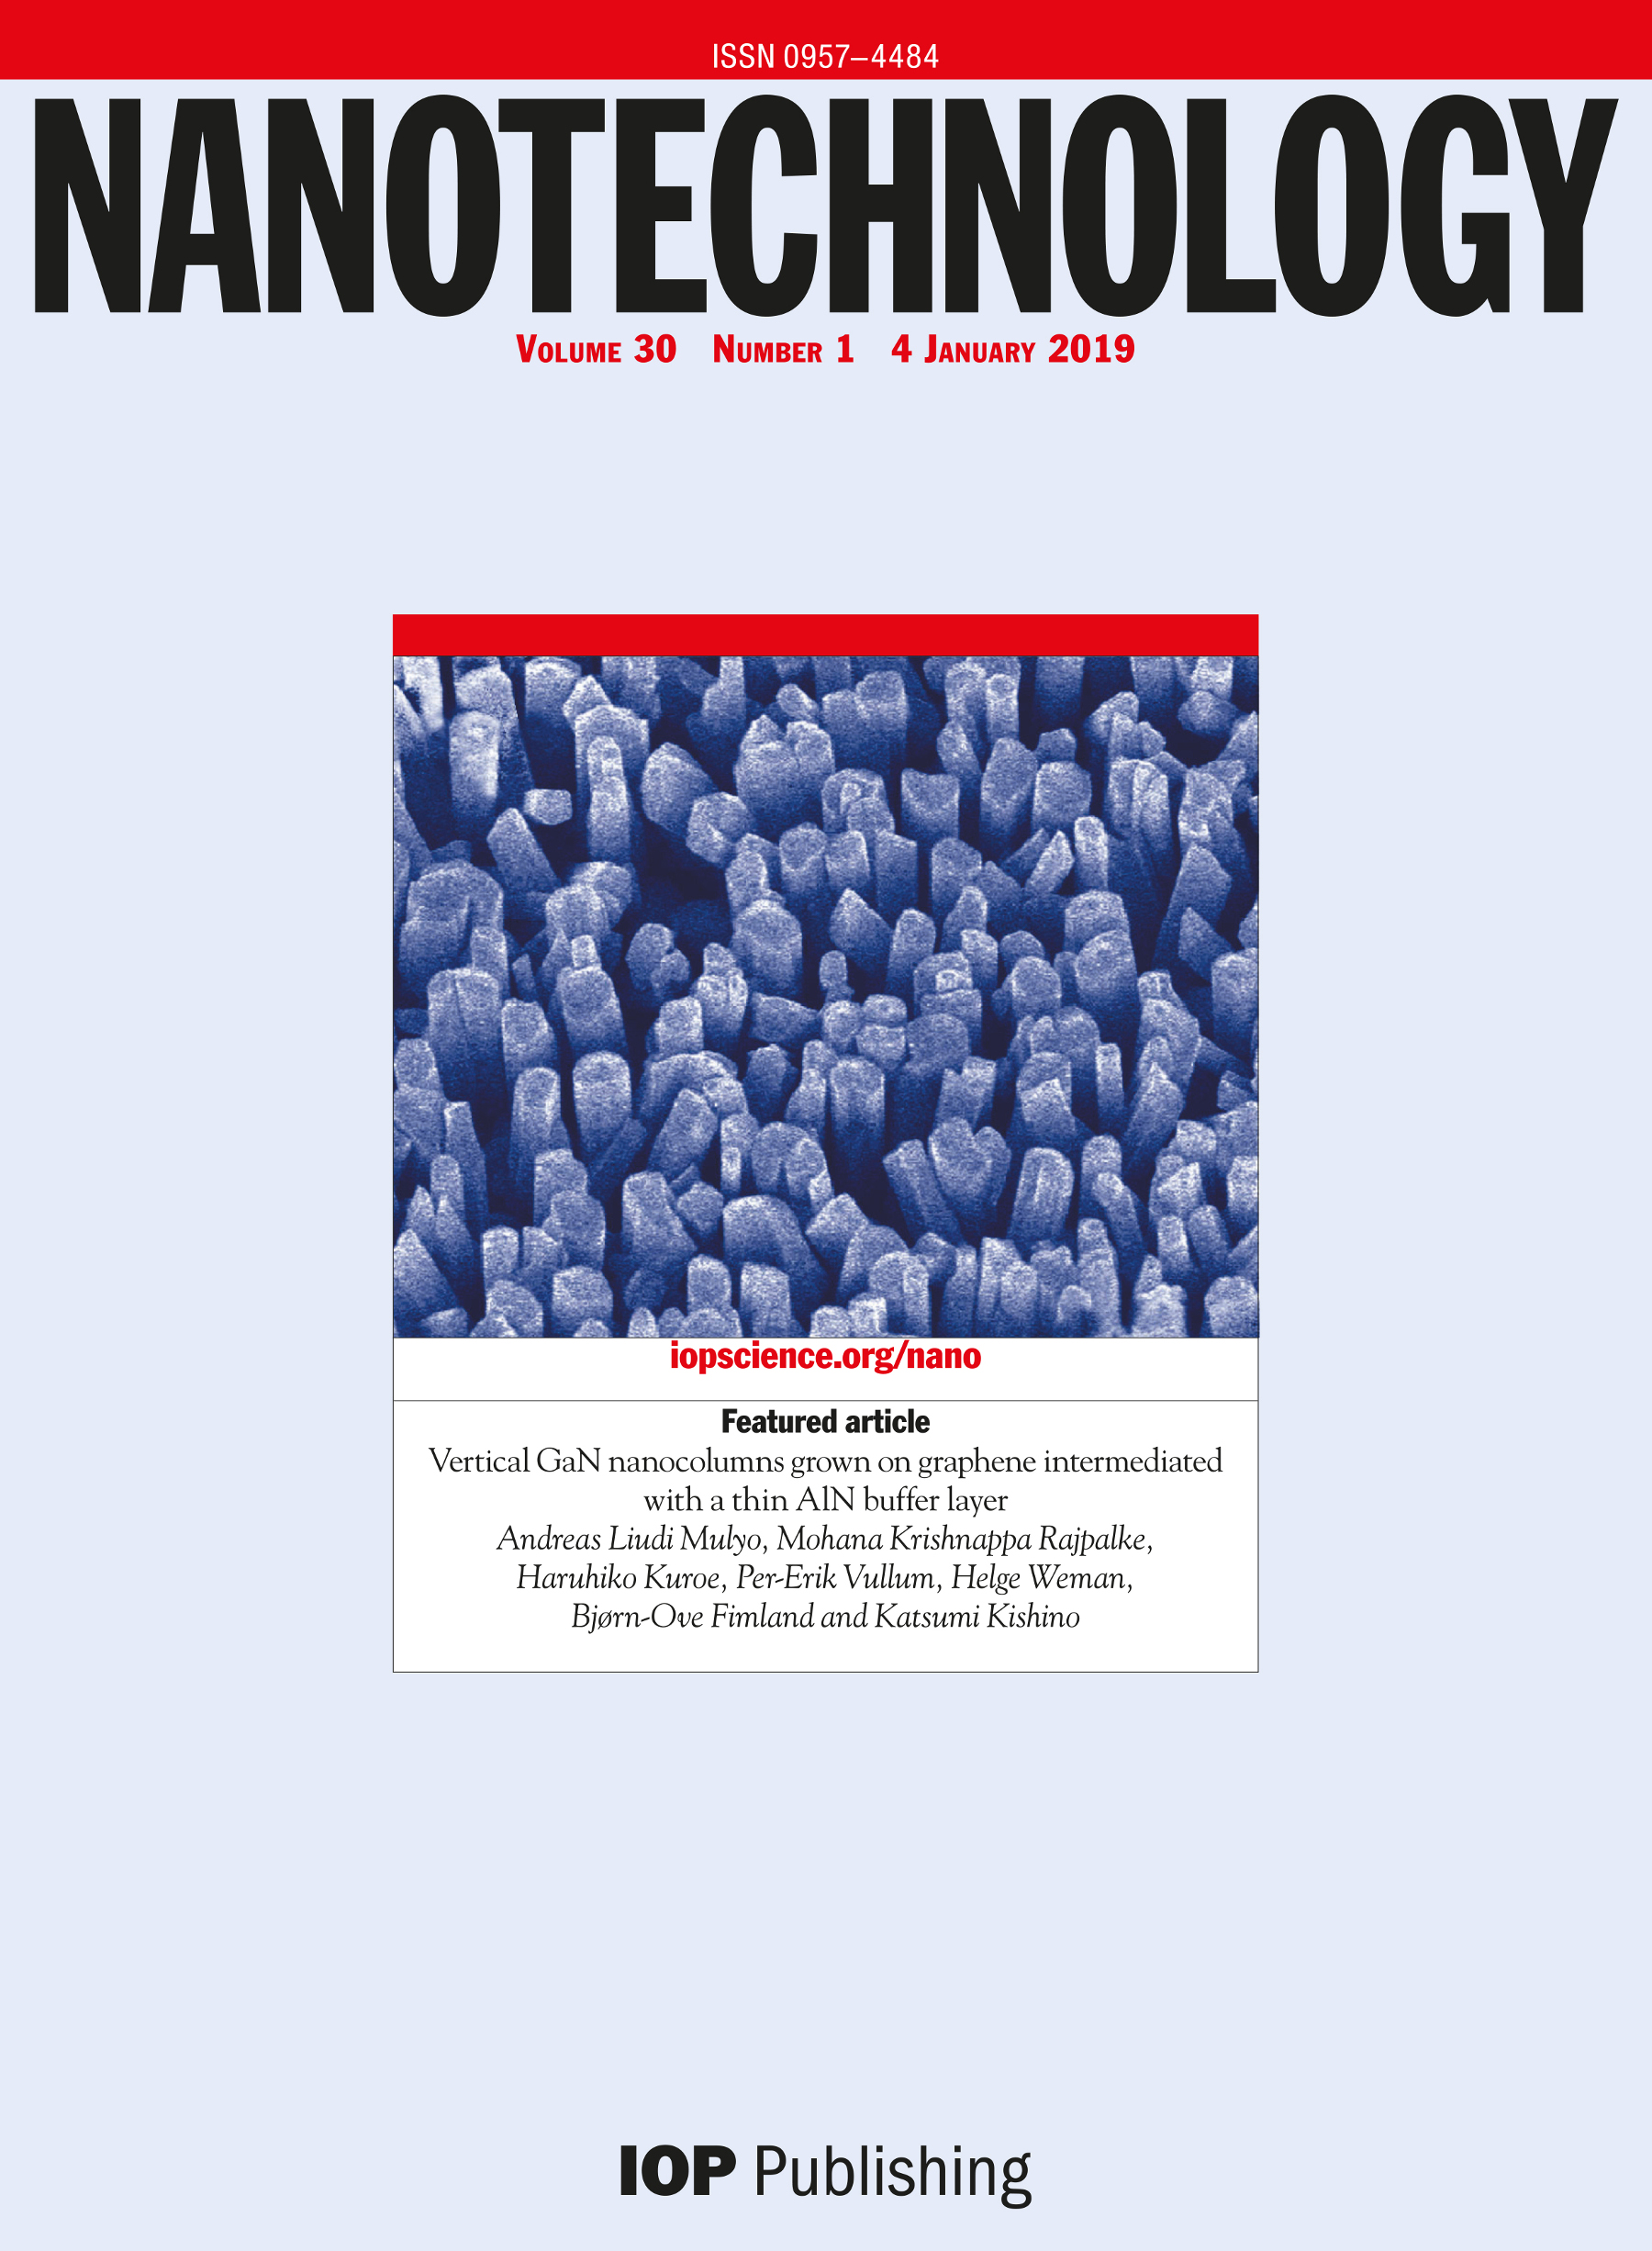
\includegraphics[width=\textwidth]{figures/EN6xzaWWAAEHOBt.jpg}
    \caption[Cover image/featured article in Nanotechnology]{Our work published in Nanotechnology was selected as a cover image/featured article for the first issue of 2019 (4 January).}
    \label{fig:coverimage}
\end{figure}
 
\newpage
 
{\color{sophia} \small \bfseries \fontfamily{bch} \selectfont \scshape \noindent Conference participation (presentations)} \\

\noindent Name of the author with \textsuperscript{\textdagger} indicates the presenter. Half of the past meeting records (i.e., conference websites or pdf files of the conference programs) are still accessible online, and unfortunately half of them are no longer active (as of December 03 2020). For the latter, reader might notice that they are linked via \href{http://web.archive.org}{Internet Archive} or \href{https://author.github.io}{my personal website}.

\begin{enumerate}[wide=0em, leftmargin=*, itemsep=3pt, labelsep=0.5em, widest=99, label={[\arabic*]}]

    \item \textbf{Author 1\textsuperscript{\textdagger}}, Author 2, Author 3, Author 4, Author 5, and Author 6. \textit{Title of the conference}. \textcolor{sophia}{Contributed talk} at \href{https://andreasliudimulyo.github.io/file/past-conferences/ISSLED_2017_Final_Program.pdf#page=17}{The 11th International Symposium on Semiconductor Light Emitting Devices (ISSLED 2017), Banff, Canada, October 08-12 2017}.
    
    \item Author 1\textsuperscript{\textdagger}, \textbf{Author 2}, Author 3, Author 4, Author 5, and Author 6. \textit{Title of the conference}. \textcolor{sophia}{Contributed talk} at \href{https://andreasliudimulyo.github.io/file/past-conferences/2017Nano@NTNU.pdf#page=4}{Nano@NTNU Symposium, Trondheim, Norway, December 06-07 2017}.
    
    \item \textbf{Author 1\textsuperscript{\textdagger}}, Author 2, Author 3, Author 4, Author 5, and Author 6. \textit{Title of the conference}. \textcolor{sophia}{Poster presentation} at \textcolor{ntnu}{Nano@NTNU Symposium, Trondheim, Norway, December 06-07 2017}. \\
    \textit{No website or pdf file of the conference program is associated with this item.}
    
    \item Author 1\textsuperscript{\textdagger}, \textbf{Author 2}, Author 3, Author 4, Author 5, Author 6, Author 7, and Author 8. \textit{Title of the conference}. \textcolor{sophia}{Contributed talk} at \href{https://andreasliudimulyo.github.io/file/past-conferences/NWW2018-Detailed-Preliminary-Program.pdf#page=20}{Nanowire Week, Hamilton, Canada, June 11-15 2018}.
    
    \item Author 1, \textbf{Author 2}, Author 3, Author 4, Author 5, Author 6, Author 7, and Author 8\textsuperscript{\textdagger}. \textit{Title of the conference}. \textcolor{sophia}{Poster presentation} at \href{http://web.archive.org/web/20191029062712/http://www.iwn2018.jp/IWN_AP_including_late_news.pdf#page=123}{ The International Workshop on Nitride Semiconductors, Kanazawa, Japan, November 11-16 2018}.
    
    \item \textbf{Author 1}, Author 2, Author 3, Author 4, Author 5, Author 6\textsuperscript{\textdagger}, and Author 7. \textit{Title of the conference}. \textcolor{sophia}{Poster presentation} at \href{http://web.archive.org/web/20191029062712/http://www.iwn2018.jp/IWN_AP_including_late_news.pdf#page=155}{ The International Workshop on Nitride Semiconductors, Kanazawa, Japan, November 11-16 2018}.

    \begin{sloppypar}
    \item \textbf{Author 1\textsuperscript{\textdagger}}, Author 2, Author 3, Author 4, Author 5, Author 6, and Author 7. \textit{Title of the conference}. \textcolor{sophia}{Contributed talk} at \href{http://www.nano-network.net/wp-content/uploads/2019/06/Preliminary-program-Workshop.pdf}{ The 10th annual workshop of Norwegian PhD Network on Nanotechnology for Microsystems, Tromsø, Norway, June 17-19 2019}.
    \end{sloppypar}
    
    \item \textbf{Author 1}, Author 2, Author 3, Author 4, Author 5, and Author 6\textsuperscript{\textdagger}. \textit{Title of the conference}. \textcolor{sophia}{Poster presentation} at \href{https://andreasliudimulyo.github.io/file/past-conferences/icns-13-program-web.pdf#page=9}{The 13th International Conferences on Nitride Semiconductors, Bellevue, Washington (Seattle), USA, July 07-12 2019}.
    
\end{enumerate}
%%% Copyright permissions

\chapter[Copyright permissions]{Copyright permissions}

\markboth{Copyright permissions}%
{Copyright permissions}

\regularsection
\headerregularsection

Below is the complete list of the copyright figures shown in this Doctoral thesis, mainly from chapter 1 to chapter 4.

\begin{itemize} [wide=0em, leftmargin=*, label=\adforn{74}] % , itemsep=0.7pt, parsep=0.7pt, label=\small\ding{110} 121, 122, 117, 118, 110, 111, 113, 114, 212]

    % \bibliographystyle{unsrtnat-mod}
    % \nobibliography{references}
    
    % % https://tex.stackexchange.com/questions/129811/file-ended-error-when-using-nobibliography
    % % https://tex.stackexchange.com/questions/142985/using-bibentry-to-insert-reference-in-text-and-omit-the-list-of-references-at-th
    % % https://tex.stackexchange.com/questions/33008/what-is-the-most-convenient-way-to-create-annotated-bibliographies-e-g-in-a-li
    
    % % i don't understand why it does not work here, especially with the similar pattern as of last point
    % % in any case, if it the code works, it will display "cit. on p." (or other declaration in the PREMABLE), which is unwanted here. So, manual is the only way.
    % % this will be used only for comparison
    % % UPDATE 20201211:
    % % it seems that bibentry does not work properly (annoying error messages) when the bibentry is used in the main text (in condition where backref of hyperref is activated).
    % % see:
    % % https://comp.text.tex.narkive.com/x2PWbp7j/backref-and-bibentry-conflict
    % % possible way to solve, but I can't implement them: 
    % % http://qianglee.blogspot.com/2006/08/make-bibentry-compatible-with-backref.html

    \item \ref{fig:figures/paper-iv/fig-1}\mynote{\pcol{page} \colpageref{fig:figures/paper-iv/fig-1}}is adapted with permission from: \\ A. Liudi Mulyo. \href{https://www.nature.com/articles/s41598-019-55424-z}{The influence of AlN buffer layer on the growth of self-assembled GaN nanocolumns on graphene}. \textit{Scientific Reports} \textbf{10}, 853 (2020). \\ Copyright \copyright \ 2020 Liudi Mulyo.
    
    \item \ref{fig:figures/paper-iv/fig-2}\mynote{\pcol{page} \colpageref{fig:figures/paper-iv/fig-2}}is adapted with permission from: \\ A. Liudi Mulyo. \href{https://www.nature.com/articles/s41598-019-55424-z}{The influence of AlN buffer layer on the growth of self-assembled GaN nanocolumns on graphene}. \textit{Scientific Reports} \textbf{10}, 853 (2020). \\ Copyright \copyright \ 2020 Liudi Mulyo.
    
    \item \ref{fig:figures/paper-iv/fig-3}\mynote{\pcol{page} \colpageref{fig:figures/paper-iv/fig-3}}is adapted with permission from: \\ A. Liudi Mulyo. \href{https://www.nature.com/articles/s41598-019-55424-z}{The influence of AlN buffer layer on the growth of self-assembled GaN nanocolumns on graphene}. \textit{Scientific Reports} \textbf{10}, 853 (2020). \\ Copyright \copyright \ 2020 Liudi Mulyo.
    
    \item \ref{fig:figures/paper-iv/fig-4}\mynote{\pcol{page} \colpageref{fig:figures/paper-iv/fig-4}}is adapted with permission from: \\ A. Liudi Mulyo. \href{https://www.nature.com/articles/s41598-019-55424-z}{The influence of AlN buffer layer on the growth of self-assembled GaN nanocolumns on graphene}. \textit{Scientific Reports} \textbf{10}, 853 (2020). \\ Copyright \copyright \ 2020 Liudi Mulyo.

    \item \ref{fig:figures/paper-iv/fig-5}\mynote{\pcol{page} \colpageref{fig:figures/paper-iv/fig-5}}is adapted with permission from: \\ A. Liudi Mulyo. \href{https://www.nature.com/articles/s41598-019-55424-z}{The influence of AlN buffer layer on the growth of self-assembled GaN nanocolumns on graphene}. \textit{Scientific Reports} \textbf{10}, 853 (2020). \\ Copyright \copyright \ 2020 Liudi Mulyo.

    \item \ref{fig:figures/paper-iv/fig-6}\mynote{\pcol{page} \colpageref{fig:figures/paper-iv/fig-6}}is adapted with permission from: \\ A. Liudi Mulyo. \href{https://www.nature.com/articles/s41598-019-55424-z}{The influence of AlN buffer layer on the growth of self-assembled GaN nanocolumns on graphene}. \textit{Scientific Reports} \textbf{10}, 853 (2020). \\ Copyright \copyright \ 2020 Liudi Mulyo.

    \item \ref{fig:figures/paper-iv/fig-7}\mynote{\pcol{page} \colpageref{fig:figures/paper-iv/fig-7}}is adapted with permission from: \\ A. Liudi Mulyo. \href{https://www.nature.com/articles/s41598-019-55424-z}{The influence of AlN buffer layer on the growth of self-assembled GaN nanocolumns on graphene}. \textit{Scientific Reports} \textbf{10}, 853 (2020). \\ Copyright \copyright \ 2020 Liudi Mulyo.
        
\end{itemize}
%% Index

\cleardoublepage\phantomsection % to fix wrong hyperref to \chapter*{print index}
% \setcounter{page}{1}
% \renewcommand{\thepage}{I-\arabic{page}}

% \markboth{Index}% not necessary for "\renewenvironment{theindex} % require"
% {Index}

% \regularsection % not necessary as there is no section and subsection here

\setcounter{page}{1}
\renewcommand{\thepage}{M-\arabic{page}}

% ==============================

\headerregularsection % it appears that "index" has a function of "\Makeuppercase" within their heading/footer. so to solve this, in practice, it is similar with reference, meaning the same way to tackle this: by issuing "\headerspecialsection"

% % OR

% \headerspecialsection % not necessary (?) for "\renewenvironment{theindex} % require"

% % err.... after several runs, the header/footer for "index" is slightly bit complicated 
% % you need to run a few times to see the changes
% % these two functions are not completely useless

% ==============================

% % run with "\renewenvironment{theindex} % require "\chapter{Index} \begin{multicols}{2} \printindex \end{multicols}" in the preamble
% \chapter{Index} 
% \begin{multicols}{2}
% \printindex
% \end{multicols}

% % OR

% run with "\renewenvironment{theindex} % require only "\printindex" in the backmatter/index.tex" in the preamble
{\hypersetup{linkcolor=sophia}
\printindex
}
% Multi-column with "\renewenvironment{theindex}" in the preamble : https://latex.org/forum/viewtopic.php?t=1735
% other alternatives are available there too

% how to index
% https://withoutbullshit.com/blog/the-sublime-joy-of-making-a-book-index-indexing
% https://writingcooperative.com/five-step-process-for-writing-a-book-index-9e2e5d763302

% to-do list in the future:
% thumb indices --> https://data.math.au.dk/latex/bog/version3/beta/ltxb-2011-09-13-20-10.pdf#page=459
% first and last word in the header --> https://tex.stackexchange.com/questions/26122/indexing-an-interval-of-words-on-top-of-every-page

% \cleardoublepage % intentionally put Colophon in the even page -> ignore the following error 
% % "Package marginnote Warning: Consecutive odd pages found. Note, it is not recommended to use consecutive odd pages in a double-ended document. The pages of your document should always be a sequence: odd-even-odd-even-... Maybe you've forgotten a \cleardoublepage before changing the page numbering on page End-1."
\WarningFilter{marginnote}{Consecutive odd pages found}

\pagestyle{empty}

\setcounter{page}{1}
\renewcommand{\thepage}{End-\arabic{page}}

\hfill

\vfill

{

\begin{adjustwidth}{-1mm}{1cm} % 
{\noindent \color{sophia} 
\small
\bfseries \fontfamily{bch} \selectfont \scshape Colophon} \vspace{4mm}
\end{adjustwidth}

\noindent This thesis was typeset using \LaTeX \ and the \texttt{book} documentclass. Main text is contained within the dimension of 115 mm (width)/197.2 mm (length), where the horizontal (top:bottom) and vertical (left:right) margin ratios are 1:1. The width of the margin notes is 12 mm. Style of this thesis is inspired by Friedrich Wiemer's thesis \textit{Security Arguments and Tool-based Design of Block Ciphers} [\url{https://hss-opus.ub.rub.de/opus4/frontdoor/deliver/index/docId/7044/file/diss.pdf}]. \\

\noindent Sebastian Kosch's \textit{Crimson} [\url{https://github.com/skosch/Crimson}] is set as the running text (11 pt) typeface. Matthew Carter’s \textit{Charter} acts as the title (14.4 pt), section (10 pt), subsection (10 pt), and header (8 pt) typefaces. Hermann Zapf's \textit{Palatino} serves as the page (9 pt) typeface. Christian Robertson's \textit{Roboto} [\url{https://tug.org/FontCatalogue/roboto/}] is utilized for the figure caption (8 pt) typeface. Libertine Open Fonts Project's \textit{Linux Libertine} [\url{https://tug.org/FontCatalogue/linuxlibertine/}] and Linus Romer's \textit{Miama Nueva} [\url{https://tug.org/FontCatalogue/miamanueva/}] are used for math/equation (11 pt) and calligraphical (14.4 pt) typefaces. The \texttt{textgreek} package [\url{https://www.ctan.org/pkg/textgreek}] provides Greek letters in normal font (being not \textit{italicized} as in \texttt{\$math\$} mode). \\

\begin{sloppypar}
\noindent Six different color palettes exploited throughout this thesis are listed as follows: \colorbox{ntnu}{\textcolor{White}{\texttt{RGB: 0, 80, 158}}} , \colorbox{sophia}{\textcolor{White}{\texttt{RGB: 125, 0, 45}}} , \colorbox{abstractback}{\texttt{RGB: 255, 248, 220}} , \colorbox{Test}{\texttt{RGB: 231, 231, 231}} , \colorbox{heidelberg}{\textcolor{White}{\texttt{RGB: 0, 65, 120}}} , and \colorbox{Test3}{\textcolor{White}{\texttt{RGB: 128, 128, 128}}} . \\
\end{sloppypar}

\noindent The references were processed by \texttt{BibTeX/natbib} -backref option enabled- with modified \texttt{unsrtnat} bibliography style. Further details on the packages utilized to make this thesis, along with the \LaTeX \ source (template) of this thesis can be found on \url{https://andreasliudimulyo.github.io/#latex}. \\

\begin{sloppypar}
\noindent Most of the graphics in this thesis were generated using \texttt{Inkscape} [\url{https://inkscape.org}] and \texttt{Ngraph} [\url{https://forest.watch.impress.co.jp/library/software/ngraph/}].
\end{sloppypar}

\vspace{4mm}

\noindent\emph{Final Version} as of \today% \ at \ \currenttime. 
}

\end{document}
